% !TeX spellcheck = hu_HU
% !TeX encoding = UTF-8
% !TeX program = xelatex
% TODO Change language to en_GB (recommended) or en_US for English documents
\documentclass[12pt,a4paper,oneside]{report}             % Single-side
%\documentclass[11pt,a4paper,twoside,openright]{report}  % Duplex

% thanks to http://tex.stackexchange.com/a/47579/71109
\usepackage{ifxetex}
\usepackage{ifluatex}
\newif\ifxetexorluatex % a new conditional starts as false
\ifnum 0\ifxetex 1\fi\ifluatex 1\fi>0
   \xetexorluatextrue
\fi

\ifxetexorluatex
  \usepackage{fontspec}
\else
  \usepackage[T1]{fontenc}
  \usepackage[utf8]{inputenc}
  \usepackage[lighttt]{lmodern}
\fi

\usepackage[english,magyar]{babel} % Alapértelmezés szerint utoljára definiált nyelv lesz aktív, de később külön beállítjuk az aktív nyelvet.

%\usepackage{cmap}
\usepackage{amsfonts,amsmath,amssymb} % Mathematical symbols.
%\usepackage[ruled,boxed,resetcount,linesnumbered]{algorithm2e} % For pseudocodes. % beware: this is not compatible with LuaLaTeX, see http://tex.stackexchange.com/questions/34814/lualatex-and-algorithm2e
\usepackage{booktabs} % For publication quality tables for LaTeX
\usepackage{graphicx}

%\usepackage{fancyhdr}
%\usepackage{lastpage}

\usepackage{anysize}
%\usepackage{sectsty}
\usepackage{setspace} % For setting line spacing

\usepackage[unicode]{hyperref} % For hyperlinks in the generated document.
\usepackage{xcolor}
\usepackage{listings} % For source code snippets.

\usepackage[amsmath,thmmarks]{ntheorem} % Theorem-like environments.

\usepackage[hang]{caption}

\singlespacing

\newcommand{\selecthungarian}{
	\selectlanguage{magyar}
	\setlength{\parindent}{2em}
	\setlength{\parskip}{0em}
	\frenchspacing
}

\newcommand{\selectenglish}{
	\selectlanguage{english}
	\setlength{\parindent}{0em}
	\setlength{\parskip}{0.5em}
	\nonfrenchspacing
	\renewcommand{\figureautorefname}{Figure}
	\renewcommand{\tableautorefname}{Table}
	\renewcommand{\partautorefname}{Part}
	\renewcommand{\chapterautorefname}{Chapter}
	\renewcommand{\sectionautorefname}{Section}
	\renewcommand{\subsectionautorefname}{Section}
	\renewcommand{\subsubsectionautorefname}{Section}
}

\usepackage[numbers]{natbib}
\usepackage{xspace}
\usepackage{array}
\usepackage{tabularx}
\usepackage{multirow}
\usepackage{pdfpages}
\usepackage{float}
\usepackage{comment}


%TODO Set the main variables
\newcommand{\vikszerzoVezeteknev}{Veress}
\newcommand{\vikszerzoKeresztnev}{Gábor}

\newcommand{\vikkonzulensAMegszolitas}{dr.~}
\newcommand{\vikkonzulensAVezeteknev}{Zsóka}
\newcommand{\vikkonzulensAKeresztnev}{Zoltán}

\newcommand{\vikkonzulensBMegszolitas}{}
\newcommand{\vikkonzulensBVezeteknev}{}
\newcommand{\vikkonzulensBKeresztnev}{}

\newcommand{\vikkonzulensCMegszolitas}{}
\newcommand{\vikkonzulensCVezeteknev}{}
\newcommand{\vikkonzulensCKeresztnev}{}

\newcommand{\vikcim}{Keretrendszer energetikai felügyelethez} % Cím
\newcommand{\viktanszek}{\bmehit} % Tanszék
\newcommand{\vikdoktipus}{\msc} % Dokumentum típusa (\bsc vagy \msc)
\newcommand{\vikmunkatipusat}{diplomatervet} % a "hallgató nyilatkozat" részhez: szakdolgozatot vagy diplomatervet

%--------------------------------------------------------------------------------------
% TDK-specifikus változók
%--------------------------------------------------------------------------------------
\newcommand{\tdkszerzoB}{Második Szerző} % Második szerző neve; hagyd üresen, ha egyedül írtad a TDK-t.
\newcommand{\tdkev}{2014} % A dolgozat írásának éve (pl. "2014") (Ez OTDK-nál eltérhet az aktuális évtől.)

% További adatok az OTDK címlaphoz (BME-s TDK-hoz nem kell kitölteni)
\newcommand{\tdkevfolyamA}{IV} % Első szerző évfolyama, római számmal (pl. IV).
\newcommand{\tdkevfolyamB}{III} % Második szerző évfolyama, római számmal (pl. III).
\newcommand{\tdkkonzulensbeosztasA}{egyetemi tanár} % Első konzulens beosztása (pl. egyetemi docens)
\newcommand{\tdkkonzulensbeosztasB}{doktorandusz} % Második konzulens beosztása (pl. egyetemi docens)

\newcommand{\szerzoMeta}{\vikszerzoVezeteknev{} \vikszerzoKeresztnev} % egy szerző esetén
%\newcommand{\szerzoMeta}{\vikszerzoVezeteknev{} \vikszerzoKeresztnev, \tdkszerzoB} % két szerző esetén

%TODO Language configuration -- choose one
% Beállítások magyar nyelvű dolgozathoz
%--------------------------------------------------------------------------------------
% Elnevezések
%--------------------------------------------------------------------------------------
\newcommand{\bme}{Budapesti Műszaki és Gazdaságtudományi Egyetem}
\newcommand{\vik}{Villamosmérnöki és Informatikai Kar}

\newcommand{\bmehit}{Hálózati Rendszerek és Szolgáltatások Tanszék}

\newcommand{\keszitette}{Készítette}
\newcommand{\konzulens}{Konzulens}

\newcommand{\bsc}{Szakdolgozat}
\newcommand{\msc}{Diplomaterv}
\newcommand{\tdk}{TDK dolgozat}
\newcommand{\bsconlab}{BSc Önálló laboratórium}
\newcommand{\msconlabi}{MSc Önálló laboratórium 1.}
\newcommand{\msconlabii}{MSc Önálló laboratórium 2.}

\newcommand{\pelda}{Példa}
\newcommand{\definicio}{Definíció}
\newcommand{\tetel}{Tétel}

\newcommand{\bevezetes}{Bevezetés}
\newcommand{\koszonetnyilvanitas}{Köszönetnyilvánítás}
\newcommand{\fuggelek}{Függelék}

% Opcionálisan átnevezhető címek
%\addto\captionsmagyar{%
%\renewcommand{\listfigurename}{Saját ábrajegyzék cím}
%\renewcommand{\listtablename}{Saját táblázatjegyzék cím}
%\renewcommand{\bibname}{Saját irodalomjegyzék név}
%}

\newcommand{\szerzo}{\vikszerzoVezeteknev{} \vikszerzoKeresztnev}
\newcommand{\vikkonzulensA}{\vikkonzulensAMegszolitas\vikkonzulensAVezeteknev{} \vikkonzulensAKeresztnev}
\newcommand{\vikkonzulensB}{\vikkonzulensBMegszolitas\vikkonzulensBVezeteknev{} \vikkonzulensBKeresztnev}
\newcommand{\vikkonzulensC}{\vikkonzulensCMegszolitas\vikkonzulensCVezeteknev{} \vikkonzulensCKeresztnev}

\newcommand{\selectthesislanguage}{\selecthungarian}

\bibliographystyle{huplain}

\def\lstlistingname{lista}

\newcommand{\appendixnumber}{6}  % a fofejezet-szamlalo az angol ABC 6. betuje (F) lesz

% Settings for English documents
%%--------------------------------------------------------------------------------------
% Elnevezések
%--------------------------------------------------------------------------------------
\newcommand{\bme}{Budapest University of Technology and Economics}
\newcommand{\vik}{Faculty of Electrical Engineering and Informatics}

\newcommand{\bmehit}{Department of Networked Systems and Services}

\newcommand{\keszitette}{Author}
\newcommand{\konzulens}{Advisor}

\newcommand{\bsc}{Bachelor's Thesis}
\newcommand{\msc}{Master's Thesis}
\newcommand{\tdk}{Scientific Students' Association Report}
\newcommand{\bsconlab}{BSc Project Laboratory}
\newcommand{\msconlabi}{MSc Project Laboratory 1}
\newcommand{\msconlabii}{MSc Project Laboratory 2}

\newcommand{\pelda}{Example}
\newcommand{\definicio}{Definition}
\newcommand{\tetel}{Theorem}

\newcommand{\bevezetes}{Introduction}
\newcommand{\koszonetnyilvanitas}{Acknowledgements}
\newcommand{\fuggelek}{Appendix}

% Optional custom titles
%\addto\captionsenglish{%
%\renewcommand*{\listfigurename}{Your list of figures title}
%\renewcommand*{\listtablename}{Your list of tables title}
%\renewcommand*{\bibname}{Your bibliography title}
%}

\newcommand{\szerzo}{\vikszerzoKeresztnev{} \vikszerzoVezeteknev}
\newcommand{\vikkonzulensA}{\vikkonzulensAMegszolitas\vikkonzulensAKeresztnev{} \vikkonzulensAVezeteknev}
\newcommand{\vikkonzulensB}{\vikkonzulensBMegszolitas\vikkonzulensBKeresztnev{} \vikkonzulensBVezeteknev}
\newcommand{\vikkonzulensC}{\vikkonzulensCMegszolitas\vikkonzulensCKeresztnev{} \vikkonzulensCVezeteknev}

\newcommand{\selectthesislanguage}{\selectenglish}

\bibliographystyle{plainnat}

\newcommand{\ie}{i.e.\@\xspace}
\newcommand{\Ie}{I.e.\@\xspace}
\newcommand{\eg}{e.g.\@\xspace}
\newcommand{\Eg}{E.g.\@\xspace}
\newcommand{\etal}{et al.\@\xspace}
\newcommand{\etc}{etc.\@\xspace}
\newcommand{\vs}{vs.\@\xspace}
\newcommand{\viz}{viz.\@\xspace} % videlicet
\newcommand{\cf}{cf.\@\xspace} % confer
\newcommand{\Cf}{Cf.\@\xspace}
\newcommand{\wrt}{w.r.t.\@\xspace} % with respect to
\newcommand{\approximately}{approx.\@\xspace}

\newcommand{\appendixnumber}{1}  % a fofejezet-szamlalo az angol ABC 1. betuje (A) lesz


%--------------------------------------------------------------------------------------
% Page layout setup
%--------------------------------------------------------------------------------------
% we need to redefine the pagestyle plain
% another possibility is to use the body of this command without \fancypagestyle
% and use \pagestyle{fancy} but in that case the special pages
% (like the ToC, the References, and the Chapter pages)remain in plane style

\pagestyle{plain}
\marginsize{35mm}{25mm}{15mm}{15mm}

\setcounter{tocdepth}{3}
%\sectionfont{\large\upshape\bfseries}
\setcounter{secnumdepth}{3}

\sloppy % Margón túllógó sorok tiltása.
\widowpenalty=10000 \clubpenalty=10000 %A fattyú- és árvasorok elkerülése
\def\hyph{-\penalty0\hskip0pt\relax} % Kötőjeles szavak elválasztásának engedélyezése


%--------------------------------------------------------------------------------------
% Setup hyperref package
%--------------------------------------------------------------------------------------
\hypersetup{
    % bookmarks=true,            % show bookmarks bar?
    unicode=true,              % non-Latin characters in Acrobat's bookmarks
    pdftitle={\vikcim},        % title
    pdfauthor={\szerzoMeta},    % author
    pdfsubject={\vikdoktipus}, % subject of the document
    pdfcreator={\szerzoMeta},   % creator of the document
    pdfproducer={},    % producer of the document
    pdfkeywords={},    % list of keywords (separate then by comma)
    pdfnewwindow=true,         % links in new window
    colorlinks=true,           % false: boxed links; true: colored links
    linkcolor=black,           % color of internal links
    citecolor=black,           % color of links to bibliography
    filecolor=black,           % color of file links
    urlcolor=black             % color of external links
}


%--------------------------------------------------------------------------------------
% Set up listings
%--------------------------------------------------------------------------------------
\definecolor{lightgray}{rgb}{0.95,0.95,0.95}
\lstset{
	basicstyle=\scriptsize\ttfamily, % print whole listing small
	keywordstyle=\color{black}\bfseries, % bold black keywords
	identifierstyle=, % nothing happens
	% default behavior: comments in italic, to change use
	% commentstyle=\color{green}, % for e.g. green comments
	stringstyle=\scriptsize,
	showstringspaces=false, % no special string spaces
	aboveskip=3pt,
	belowskip=3pt,
	backgroundcolor=\color{lightgray},
	columns=flexible,
	keepspaces=true,
	escapeinside={(*@}{@*)},
	captionpos=b,
	breaklines=true,
	frame=single,
	float=!ht,
	tabsize=2,
	literate=*
		{á}{{\'a}}1	{é}{{\'e}}1	{í}{{\'i}}1	{ó}{{\'o}}1	{ö}{{\"o}}1	{ő}{{\H{o}}}1	{ú}{{\'u}}1	{ü}{{\"u}}1	{ű}{{\H{u}}}1
		{Á}{{\'A}}1	{É}{{\'E}}1	{Í}{{\'I}}1	{Ó}{{\'O}}1	{Ö}{{\"O}}1	{Ő}{{\H{O}}}1	{Ú}{{\'U}}1	{Ü}{{\"U}}1	{Ű}{{\H{U}}}1
}


%--------------------------------------------------------------------------------------
% Set up theorem-like environments
%--------------------------------------------------------------------------------------
% Using ntheorem package -- see http://www.math.washington.edu/tex-archive/macros/latex/contrib/ntheorem/ntheorem.pdf

\theoremstyle{plain}
\theoremseparator{.}
\newtheorem{example}{\pelda}

\theoremseparator{.}
%\theoremprework{\bigskip\hrule\medskip}
%\theorempostwork{\hrule\bigskip}
\theorembodyfont{\upshape}
\theoremsymbol{{\large \ensuremath{\centerdot}}}
\newtheorem{definition}{\definicio}

\theoremseparator{.}
%\theoremprework{\bigskip\hrule\medskip}
%\theorempostwork{\hrule\bigskip}
\newtheorem{theorem}{\tetel}


%--------------------------------------------------------------------------------------
% Some new commands and declarations
%--------------------------------------------------------------------------------------
\newcommand{\code}[1]{{\upshape\ttfamily\scriptsize\indent #1}}
\newcommand{\doi}[1]{DOI: \href{http://dx.doi.org/\detokenize{#1}}{\raggedright{\texttt{\detokenize{#1}}}}} % A hivatkozások közt így könnyebb DOI-t megadni.

\DeclareMathOperator*{\argmax}{arg\,max}
%\DeclareMathOperator*[1]{\floor}{arg\,max}
\DeclareMathOperator{\sign}{sgn}
\DeclareMathOperator{\rot}{rot}


%--------------------------------------------------------------------------------------
% Setup captions
%--------------------------------------------------------------------------------------
\captionsetup[figure]{
	width=.75\textwidth,
	aboveskip=10pt}

\renewcommand{\captionlabelfont}{\bf}
%\renewcommand{\captionfont}{\footnotesize\it}

%--------------------------------------------------------------------------------------
% Hyphenation exceptions
%--------------------------------------------------------------------------------------
\hyphenation{Shakes-peare Mar-seilles ár-víz-tű-rő tü-kör-fú-ró-gép}


\author{\vikszerzo}
\title{\viktitle}

%--------------------------------------------------------------------------------------
% Table of contents and the main text
%--------------------------------------------------------------------------------------
\begin{document}

\pagenumbering{gobble}

%TODO These includes define guidelines -- remove these
%~~~~~~~~~~~~~~~~~~~~~~~~~~~~~~~~~~~~~~~~~~~~~~~~~~~~~~~~~~~~~~~~~~~~~~~~~~~~~~~~~~~~~~
%\selecthungarian
%--------------------------------------------------------------------------------------
% Rovid formai es tartalmi tajekoztato
%--------------------------------------------------------------------------------------

\footnotesize
\begin{center}
\large
\textbf{\Large Általános információk, a diplomaterv szerkezete}\\
\end{center}

A diplomaterv szerkezete a BME Villamosmérnöki és Informatikai Karán:
\begin{enumerate}
\item	Diplomaterv feladatkiírás
\item	Címoldal
\item	Tartalomjegyzék
\item	A diplomatervező nyilatkozata az önálló munkáról és az elektronikus adatok kezeléséről
\item	Tartalmi összefoglaló magyarul és angolul
\item	Bevezetés: a feladat értelmezése, a tervezés célja, a feladat indokoltsága, a diplomaterv felépítésének rövid összefoglalása
\item	A feladatkiírás pontosítása és részletes elemzése
\item	Előzmények (irodalomkutatás, hasonló alkotások), az ezekből levonható következtetések
\item	A tervezés részletes leírása, a döntési lehetőségek értékelése és a választott megoldások indoklása
\item	A megtervezett műszaki alkotás értékelése, kritikai elemzése, továbbfejlesztési lehetőségek
\item	Esetleges köszönetnyilvánítások
\item	Részletes és pontos irodalomjegyzék
\item	Függelék(ek)
\end{enumerate}

Felhasználható a következő oldaltól kezdődő \LaTeX diplomatervsablon dokumentum tartalma. 

A diplomaterv szabványos méretű A4-es lapokra kerüljön. Az oldalak tükörmargóval készüljenek (mindenhol 2,5~cm, baloldalon 1~cm-es kötéssel). Az alapértelmezett betűkészlet a 12 pontos Times New Roman, másfeles sorközzel, de ettől kismértékben el lehet térni, ill. más betűtípus használata is megengedett.

Minden oldalon -- az első négy szerkezeti elem kivételével -- szerepelnie kell az oldalszámnak.

A fejezeteket decimális beosztással kell ellátni. Az ábrákat a megfelelő helyre be kell illeszteni, fejezetenként decimális számmal és kifejező címmel kell ellátni. A fejezeteket decimális aláosztással számozzuk, maximálisan 3 aláosztás mélységben (pl. 2.3.4.1.). Az ábrákat, táblázatokat és képleteket célszerű fejezetenként külön számozni (pl. 2.4. ábra, 4.2. táblázat vagy képletnél (3.2)). A fejezetcímeket igazítsuk balra, a normál szövegnél viszont használjunk sorkiegyenlítést. Az ábrákat, táblázatokat és a hozzájuk tartozó címet igazítsuk középre. A cím a jelölt rész alatt helyezkedjen el.

A képeket lehetőleg rajzoló programmal készítsék el, az egyenleteket egyenlet-szerkesztő segítségével írják le (A \LaTeX~ehhez kézenfekvő megoldásokat nyújt).

Az irodalomjegyzék szövegközi hivatkozása történhet sorszámozva (ez a preferált megoldás) vagy a Harvard-rendszerben (a szerző és az évszám megadásával). A teljes lista névsor szerinti sorrendben a szöveg végén szerepeljen (sorszámozott irodalmi hivatkozások esetén hivatkozási sorrendben). A szakirodalmi források címeit azonban mindig az eredeti nyelven kell megadni, esetleg zárójelben a fordítással. A listában szereplő valamennyi publikációra hivatkozni kell a szövegben (a \LaTeX-sablon a Bib\TeX~segítségével mindezt automatikusan kezeli). Minden publikáció a szerzők után a következő adatok szerepelnek: folyóirat cikkeknél a pontos cím, a folyóirat címe, évfolyam, szám, oldalszám tól-ig. A folyóiratok címét csak akkor rövidítsük, ha azok nagyon közismertek vagy nagyon hosszúak. Internetes hivatkozások megadásakor fontos, hogy az elérési út előtt megadjuk az oldal tulajdonosát és tartalmát (mivel a link egy idő után akár elérhetetlenné is válhat), valamint az elérés időpontját.

\vspace{5mm}
Fontos:
\begin{itemize}
	\item A szakdolgozatkészítő / diplomatervező nyilatkozata (a jelen sablonban szereplő szövegtartalommal) kötelező előírás, Karunkon ennek hiányában a szakdolgozat/diplomaterv nem bírálható és nem védhető!
	\item Mind a dolgozat, mind a melléklet maximálisan 15~MB méretű lehet!
\end{itemize}

\vspace{5mm}
\begin{center}
Jó munkát, sikeres szakdolgozatkészítést, ill. diplomatervezést kívánunk!
\end{center}

\normalsize
\selectthesislanguage
 Csak a guidelineok, he megakarom nézni
%%--------------------------------------------------------------------------------------
% Feladatkiiras (a tanszeken atveheto, kinyomtatott valtozat)
%--------------------------------------------------------------------------------------
\clearpage
\begin{center}
\large
\textbf{FELADATKIÍRÁS}\\
\end{center}

A feladatkiírást a tanszéki adminisztrációban lehet átvenni, és a leadott munkába eredeti, tanszéki pecséttel ellátott és a tanszékvezető által aláírt lapot kell belefűzni (ezen oldal \emph{helyett}, ez az oldal csak útmutatás). Az elektronikusan feltöltött dolgozatban már nem kell beleszerkeszteni ezt a feladatkiírást.
 %Alatta PDF-ként benen van
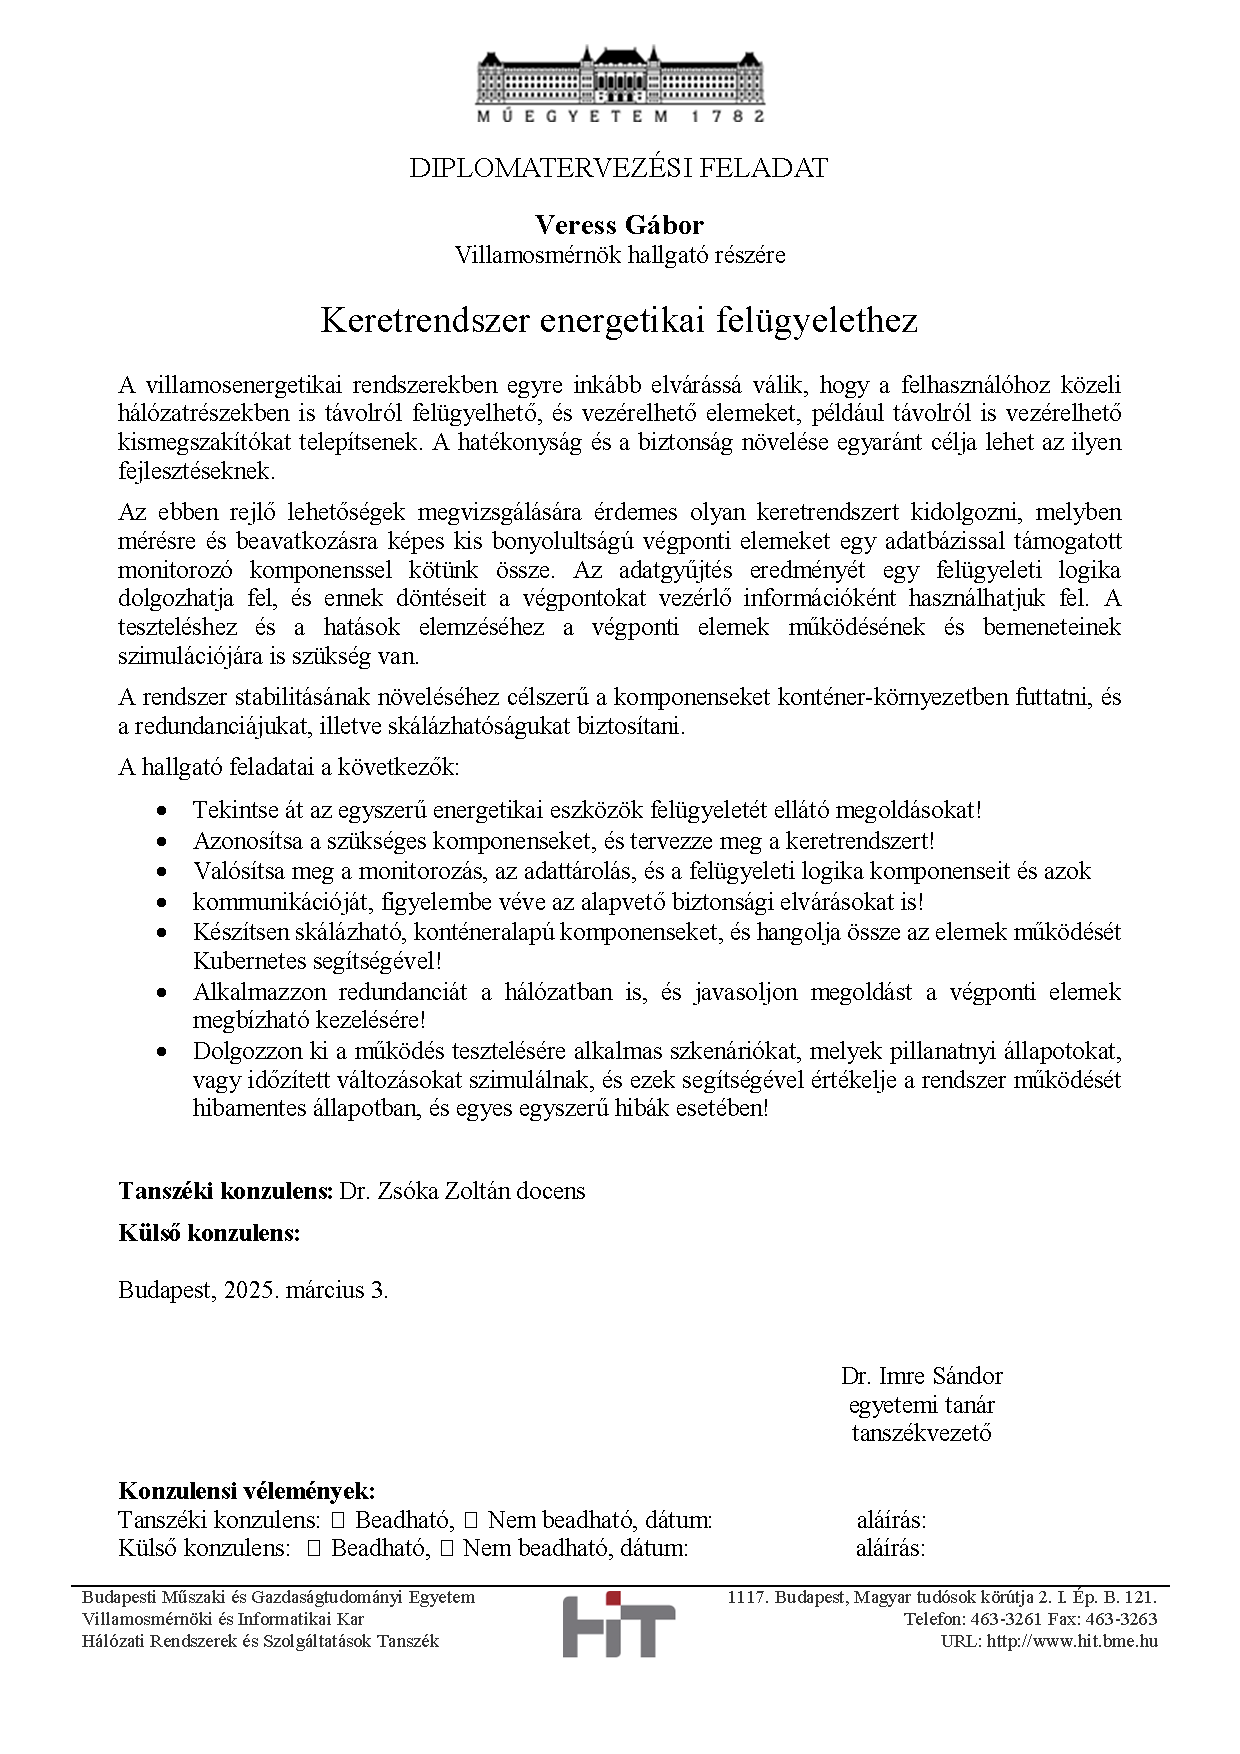
\includepdf{include/feladat.pdf}

\selectthesislanguage

%TODO Titlepage -- choose one from below
%~~~~~~~~~~~~~~~~~~~~~~~~~~~~~~~~~~~~~~~~~~~~~~~~~~~~~~~~~~~~~~~~~~~~~~~~~~~~~~~~~~~~~~
\hypersetup{pageanchor=false}
%--------------------------------------------------------------------------------------
%	The title page
%--------------------------------------------------------------------------------------
\begin{titlepage}
\begin{center}

\includegraphics[width=60mm,keepaspectratio]{figures/bme_logo.pdf}\\
\vspace{0.3cm}
\textbf{\bme}\\
\textmd{\vik}\\
\textmd{\viktanszek}\\[5cm]

\vspace{0.4cm}
{\huge \bfseries \vikcim}\\[0.8cm]
\vspace{0.5cm}
\textsc{\Large \vikdoktipus}\\[4cm]

{
	\renewcommand{\arraystretch}{0.85}
	\begin{tabular}{cc}
	 \makebox[7cm]{\emph{\keszitette}} & \makebox[7cm]{\emph{\konzulens}} \\ \noalign{\smallskip}
	 \makebox[7cm]{\szerzo} & \makebox[7cm]{\vikkonzulensA} \\
	  & \makebox[7cm]{\vikkonzulensB} \\
	  & \makebox[7cm]{\vikkonzulensC} \\
	\end{tabular}
}

\vfill
{\large \today}
\end{center}
\end{titlepage}
\hypersetup{pageanchor=false}

		   % Szakdolgozat/Diplomaterv címlap
%%% TDK címlap
\begin{titlepage}
  \begin{center}  
  
\includegraphics[width=7cm]{./figures/bme_logo.pdf}
  \vspace{0.3cm}
  
  \bme \\
  \vik \\
  \viktanszek \\
  \vspace{5cm}
  
  \huge {\vikcim}
  \vspace{1.5cm}
  
  \large {\textbf{\tdk}}
  \vfill
    
  {\Large 
  	\keszitette: \\ \vspace{0.3cm}
  	\szerzo \\
	\tdkszerzoB \\
  	\vspace{1.5cm}
  	\konzulens: \\ \vspace{0.3cm}
  	\vikkonzulensA \\
  	\vikkonzulensB \\
  }
  
  \vspace{2cm}
  \large {\tdkev}
 \end{center}
\end{titlepage}
%% Címlap vége
	% TDK címlap
%%% OTDK külső címlap
\begin{titlepage}
  	$\;$ 
	\vspace{5cm}
	
	\begin{center}
	\Huge
	\textbf{TDK-dolgozat}\let\thefootnote\relax\footnote{A dolgozat bemutatását a XXXXXXXXX  ``Lorem ipsum dolor sit amet'' című program támogatta.}
	\end{center}
	
	\vspace{13cm}
	
	\Large
	\hspace{8cm} \szerzo
	
	\hspace{8cm} \tdkszerzoB
	
	\hspace{8cm} \tdkev.
\end{titlepage}

\newpage
\thispagestyle{empty}


%% OTDK belső címlap
\begin{titlepage}
  \begin{center}  
  
\includegraphics[width=7cm]{./figures/bme_logo.pdf}
  \vspace{0.3cm}
  
  \bme \\
  \vik \\
  \viktanszek \\
  \vspace{3.5cm}
  
  \huge {\vikcim}
  \vspace{1.5cm}
  
  \large {\textbf{\vikdoktipus}}
  \vfill
    
  {\Large 
  	{\large \keszitette:} \\ \vspace{0.2cm}
  	\szerzo \\ \tdkevfolyamA. évfolyam \\
	\vspace{0.5cm}
	\tdkszerzoB \\ \tdkevfolyamB. évfolyam \\
  	\vspace{1.5cm}
  	{\large \konzulens:} \\ \vspace{0.2cm}
  	\vikkonzulensA,\\ \tdkkonzulensbeosztasA \\
  	\vspace{0.5cm}
  	\vikkonzulensB,\\ \tdkkonzulensbeosztasB \\
  }
  
  \vspace{2cm}
  \large {\tdkev.}
  
 \end{center}
\end{titlepage}   % OTDK címlap


% Table of Contents
%~~~~~~~~~~~~~~~~~~~~~~~~~~~~~~~~~~~~~~~~~~~~~~~~~~~~~~~~~~~~~~~~~~~~~~~~~~~~~~~~~~~~~~
\tableofcontents\vfill


% Declaration and Abstract
%~~~~~~~~~~~~~~~~~~~~~~~~~~~~~~~~~~~~~~~~~~~~~~~~~~~~~~~~~~~~~~~~~~~~~~~~~~~~~~~~~~~~~~
\selectlanguage{magyar}
\pagenumbering{gobble}
%--------------------------------------------------------------------------------------
% Nyilatkozat
%--------------------------------------------------------------------------------------
\begin{center}
\large
\textbf{HALLGATÓI NYILATKOZAT}\\
\end{center}

Alulírott \emph{\vikszerzoVezeteknev{} \vikszerzoKeresztnev}, szigorló hallgató kijelentem, hogy ezt a \vikmunkatipusat{} meg nem engedett segítség nélkül, saját magam készítettem, csak a megadott forrásokat (szakirodalom, eszközök stb.) használtam fel. Minden olyan részt, melyet szó szerint, vagy azonos értelemben, de átfogalmazva más forrásból átvettem, egyértelműen, a forrás megadásával megjelöltem.

Hozzájárulok, hogy a jelen munkám alapadatait (szerző(k), cím, angol és magyar nyelvű tartalmi kivonat, készítés éve, konzulens(ek) neve) a BME VIK nyilvánosan hozzáférhető elektronikus formában, a munka teljes szövegét pedig az egyetem belső hálózatán keresztül (vagy autentikált felhasználók számára) közzétegye. Kijelentem, hogy a benyújtott munka és annak elektronikus verziója megegyezik. Dékáni engedéllyel titkosított diplomatervek esetén a dolgozat szövege csak 3 év eltelte után válik hozzáférhetővé.

\begin{flushleft}
\vspace*{1cm}
Budapest, \today
\end{flushleft}

\begin{flushright}
 \vspace*{1cm}
 \makebox[7cm]{\rule{6cm}{.4pt}}\\
 \makebox[7cm]{\emph{\vikszerzoVezeteknev{} \vikszerzoKeresztnev}}\\
 \makebox[7cm]{hallgató}
\end{flushright}
\thispagestyle{empty}

\vfill
\clearpage
\thispagestyle{empty} % an empty page

\selectthesislanguage
 %TODO Hallgatói nyilatkozat -- TDK és OTDK esetén törlendő!
%\pagenumbering{roman}
\setcounter{page}{1}

\selecthungarian

%----------------------------------------------------------------------------
% Abstract in Hungarian
%----------------------------------------------------------------------------
\chapter*{Kivonat}\addcontentsline{toc}{chapter}{Kivonat}

Jelen dokumentum egy diplomaterv sablon, amely formai keretet ad a BME Villamosmérnöki és Informatikai Karán végző hallgatók által elkészítendő szakdolgozatnak és diplomatervnek. A sablon használata opcionális. Ez a sablon \LaTeX~alapú, a \emph{TeXLive} \TeX-implementációval és a PDF-\LaTeX~fordítóval működőképes.


\vfill
\selectenglish


%----------------------------------------------------------------------------
% Abstract in English
%----------------------------------------------------------------------------
\chapter*{Abstract}\addcontentsline{toc}{chapter}{Abstract}

This document is a \LaTeX-based skeleton for BSc/MSc~theses of students at the Electrical Engineering and Informatics Faculty, Budapest University of Technology and Economics. The usage of this skeleton is optional. It has been tested with the \emph{TeXLive} \TeX~implementation, and it requires the PDF-\LaTeX~compiler.


\vfill
\selectthesislanguage

\newcounter{romanPage}
\setcounter{romanPage}{\value{page}}
\stepcounter{romanPage}    %TODO Összefoglaló -- TDK és OTDK esetén nem kötelező



% The main part of the thesis
%~~~~~~~~~~~~~~~~~~~~~~~~~~~~~~~~~~~~~~~~~~~~~~~~~~~~~~~~~~~~~~~~~~~~~~~~~~~~~~~~~~~~~~
\pagenumbering{arabic}

%TODO import your own content
%----------------------------------------------------------------------------
\chapter{\bevezetes}
%----------------------------------------------------------------------------

A bevezető tartalmazza a diplomaterv-kiírás elemzését, történelmi előzményeit, a feladat indokoltságát (a motiváció leírását), az eddigi megoldásokat, és ennek tükrében a hallgató megoldásának összefoglalását.

A bevezető szokás szerint a diplomaterv felépítésével záródik, azaz annak rövid leírásával, hogy melyik fejezet mivel foglalkozik.

\chapter{Meglévő megoldásokkal összehasonlítása}

\section{Meglévő ipari megoldások}

\subsection{Schneider Power Monitoring Expert}

\subsubsection{Alapfunkciók}

\begin{itemize}
    \item Segít csökkenteni a meddő teljesítmény termelést és az ebből keletkező büntetéseket.
    \item Saját számlát készít, a helyi mérések alapján, hogy összehasonlítási alap legyen a számlákhoz.
    \item Segít elszámolhatóságot biztosítani alszámlázáshoz.
    \item Berendezések teljesítményét és várható élettartamát ellenőrzi.
    \item Valós idejű adatfigyelés, riasztás és energiafolyamatok vezérlése a létesítményen belül.
    \item Azonosítsa a potenciális áramminőségi problémákat a hálózatában, és értesíti erről a személyzetet.
\end{itemize}
\cite{sePME}

\begin{figure}[ht]
    \centering
    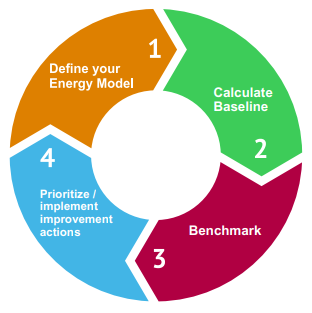
\includegraphics[width=0.3\textwidth]{figures/sePME.png}
    \caption{Schneider Electric PME model\cite{sePME}}
    \label{fig:schneider-pme}
\end{figure}

\subsubsection{Előnyök}

Az energiamérési rendszer használata átlagban 24\%-kal csökkentette a fogyasztást, 
és 30\%-al a költségeket.

Mivel folyamatos megfigyelés és  beavatkozás lehetséges, a problémák korai szakaszában orvosolhatóak így
ezeket 22\%-al lehet csökkenteni. Ez a tudatosság csökkenteni a a hiba utáni visszaállítások idejét is.
Ezenkívül segít a mögöttes problémák megtalálásában is.\cite{sePME}

\subsection{Siemens SIMATIC Energy Suite}

\subsubsection{Alapfunkciók}

A Siemens SIMATIC Energy Management rendszere integrált tehát nem csak megfigyelésre alkalmas hanem vezérlésre is. 
A már létező TIA Portal keretrendszerükbe épül és így egy helyen elérhető a többi rendszerükkel. 
Ez szintén egy moduláris és skálázható rendszer.
Megfelel az ISO 50001 szabványnak, és ez is alkalmazható terhelés figyelésre számlázásra és rendszerelemzésre,
mint az előzőleg taglalt rendszer.\cite{sieEMS}

\subsubsection{Előnyök}

\begin{itemize}
    \item Terepi szintű integráció saját és más eszközökkel. Figyelve itt az egyedi eszközökre.
    \item Gyártás szintű felügyelet. Üzem szintű energia fogyasztást lehet vele figyelni.
    \item Nagyobb rendszerekben vállalati szintű energiaelemzés, ahol több helyszín között is lehet felügyelni.
    \item Ezentúl alkalmas beavatkozásra is. Amennyiben túl nagy a fogyasztás képes fogyasztókat leválasztani távolról is akár.
\end{itemize}
\cite{sieEMS}

\begin{figure}
    \centering
    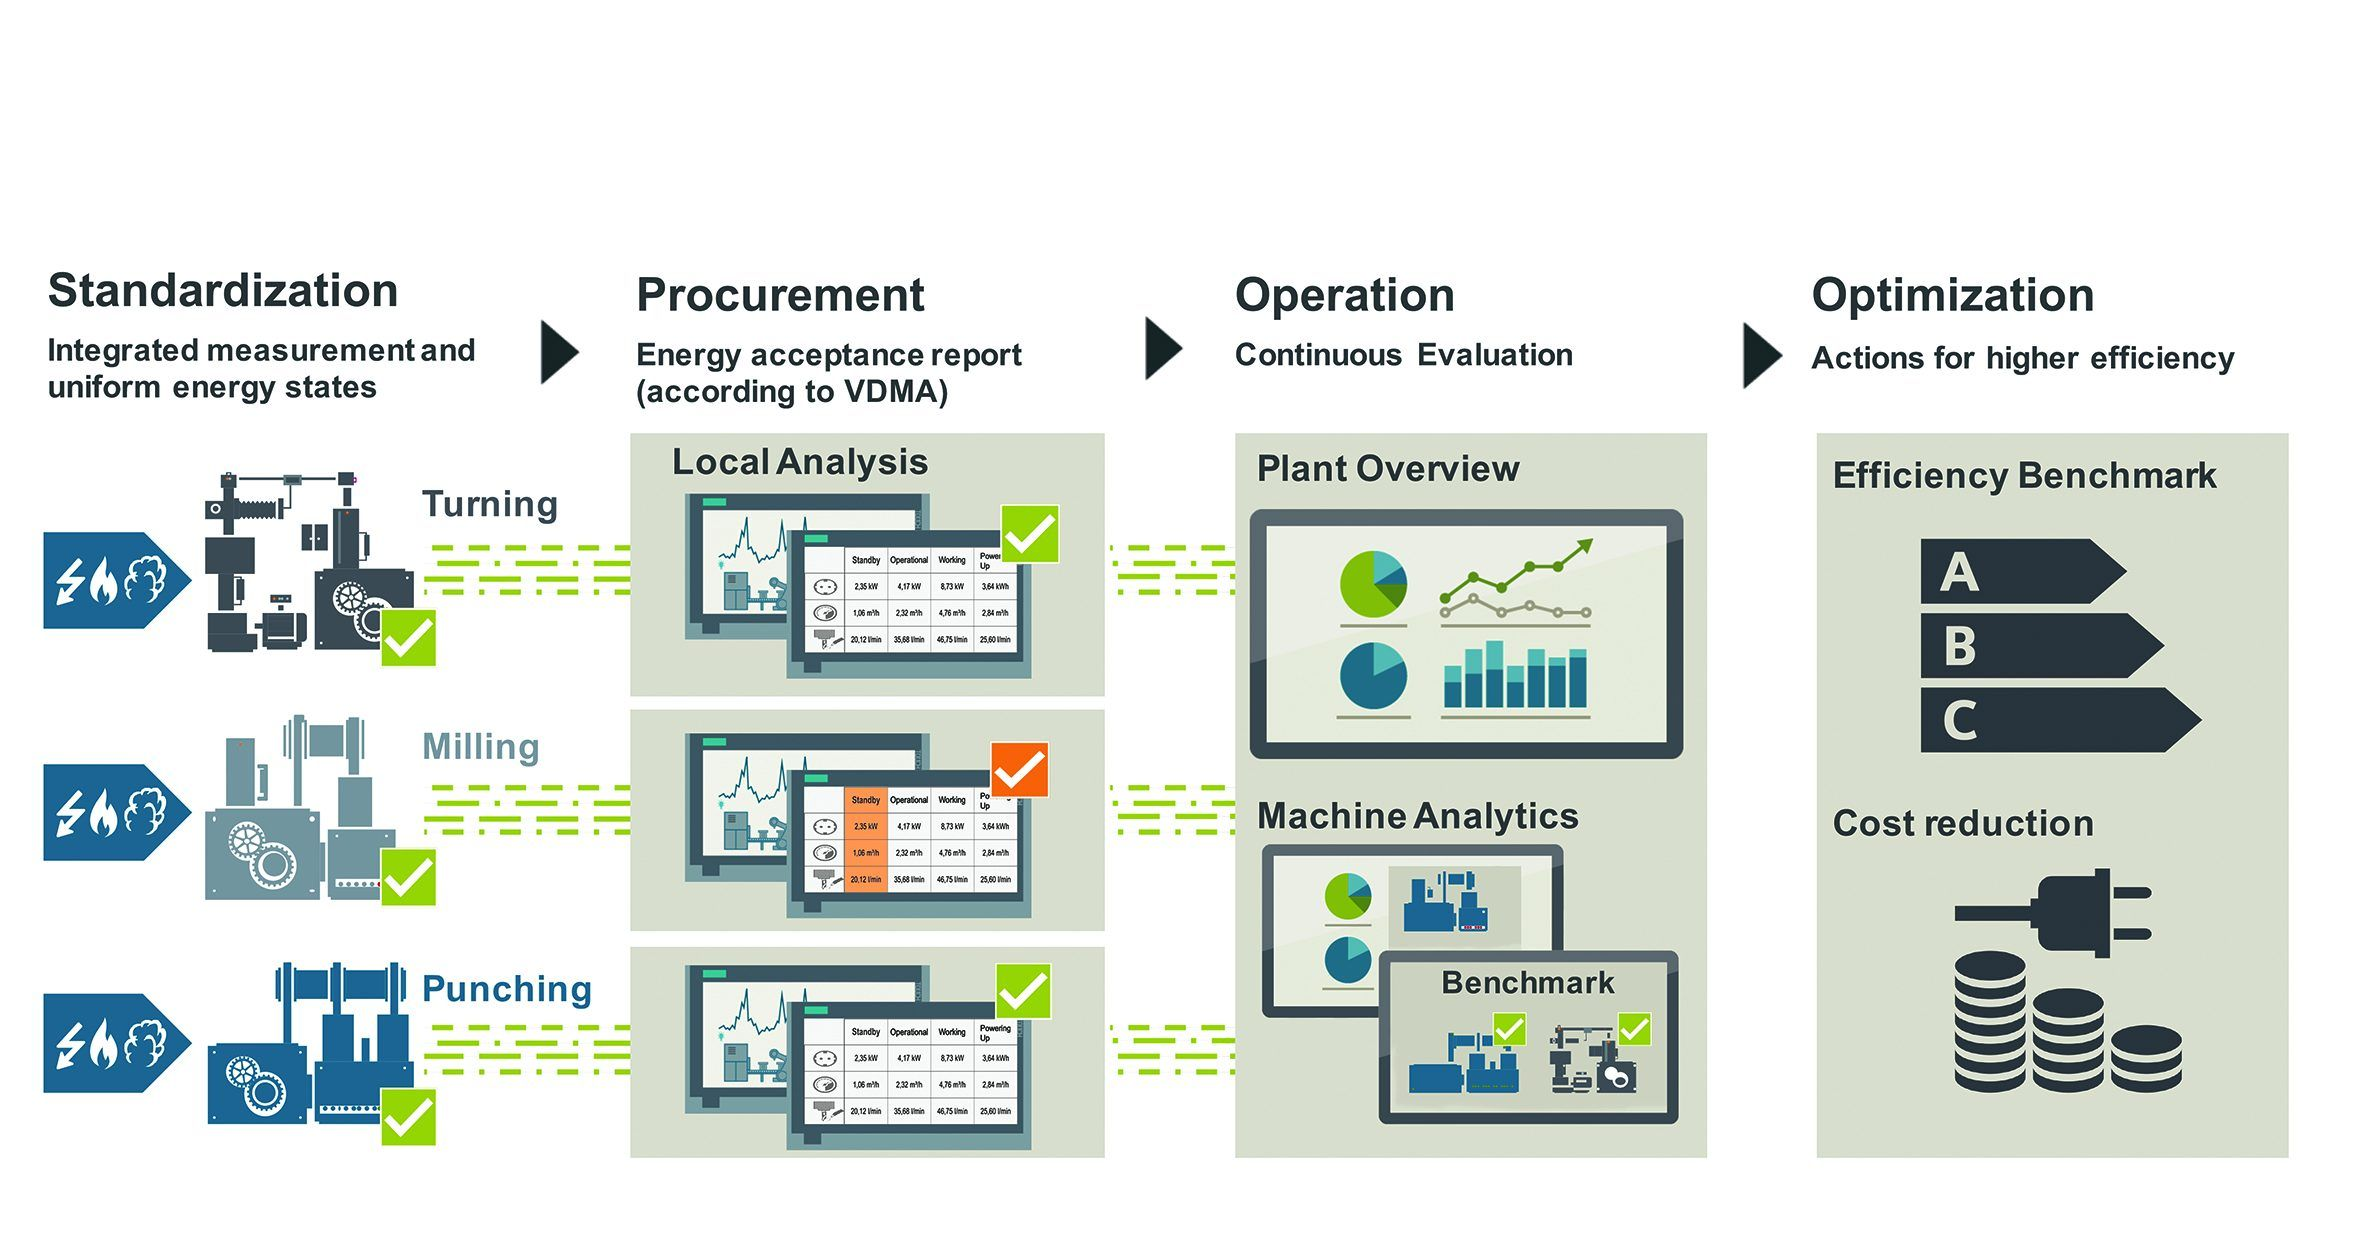
\includegraphics[width=0.8\textwidth]{figures/sieEMS.png}
    \caption{Siemens EMS model\cite{sieEMS}}
    \label{fig:siemens-ems}
\end{figure}

\section{Saját megoldás}

A dolgozatom további részében hasonló rendszer kidolgozásán szeretnék dolgozni, ami lehetőleg tartalmazza
ezeket a képességeket. Sőt lehetőleg meg is haladja őket és árban is sokkal versenyképesebb mint ezek a rendszerek.
\chapter{Keretrendszer}

\section{Szükségesség}

\section{Eszközök}

\subsection{Végpontok}

\subsubsection{ESP8266}

\subsubsection{Mért eszközök}

\subsection{Adatbázis}

\subsection{Kontroll szerver}

\section{Kommunikáció}

\subsection{Standardizált Kommunikáció}

\chapter{Komponensek megvalósítása}

\section{Végpontok}

\subsection{Autótöltő}

\subsubsection{Bevezetés}
A rendszer egy ESP8266 mikrokontroller köré épül, amely két elsődleges funkciót lát el:
\begin{itemize}
    \item Árammérés: Folyamatosan méri az autótöltők által felvett elektromos áramot. Összegyűjti és a Prometheus, 
    egy népszerű nyílt forráskódú felügyeleti rendszerrel kompatibilis formátumban jelenti ezeket a mérési adatokat, 
    hogy a rendszerben egységes adatstruktúrákat használjunk.
    \item Vezérlő interfész: Emellett olyan mechanizmust biztosít, ami Modbus parancsokon keresztül vezérli az 
    autótöltőket.
\end{itemize}

\subsubsection{Megvalósítás}
Itt az ESP8266 firmware főbb részeit elemzem.
\paragraph{WiFi és HTTP-kiszolgáló beállítása}
Kezdésnek az ESP8266 csatlakozik WiFi-re és ezzel a helyi hálózatra a megadott SSID és jelszóval. 
A csatlakozást követően az eszköz az ESP8266WebServer könyvtár segítségével inicializál egy HTTPS-kiszolgálót. 
Ez a szerver egy kijelölt porton (pl. 8663) figyel, és a /metrics végpontot teszi közzé, 
ahol közli az adatokat a központ vezérlővel.

\subsubsection{Mérési adatok elküldése}

A \texttt{sendMetricsToEndpoint()} függvény formázza a méréseket Prometheus-szerű szöveges formába. A metrikák a következőket tartalmazzák:

\begin{itemize}
  \item \textbf{esp8266\_current0}: A mért áramértéket mutatja.
  \item \textbf{esp8266\_connection}: Az ESP8266 kapcsolati állapotát jelzi, pl.: csatlakozva vagy nem.
\end{itemize}

Ez a funkció a Prometheus-kompatibilis mért érték és címkézési formátummal küldi el a mérést. 
Amikor például a vezérlő szerver lekéri a \texttt{/metrics} végpontot, a HTTPS-kiszolgáló 
\texttt{200 OK} státusszal küldi vissza ezeket a formázott metrikákat, amennyiben minden rendben ment.

\subsubsection{Main loop}
A loop() funkcióban az ESP8266 folyamatosan kezeli a bejövő HTTPS kéréseket és 30 másodpercenként 
az eszköz meghívja a queryPrometheus() függvényt, hogy frissítse az összesített metrikát. 
Ez az időszakos lekérdezési mechanizmus biztosítja, hogy a helyi mérések folyamatosan frissek 
legyenek és döntéshozatal alapjául lehessen venni őket.

\subsubsection{Kommunikáció}
A rendszer itt is a biztonságos adatátvitel érdekében minden hálózati kommunikációhoz HTTPS protokollt használ. 
A legfontosabb adatáramlások a következők:

\begin{itemize}
    \item \textbf{Mérések közzététele:} Az ESP8266 összegyűjti az aktuális méréseket, és azokat a /metrics 
    végponton olyan formátumban teszi elérhetővé, ami már alkalmas Prometheus alapú adattárolásra.
    
    \item \textbf{Visszacsatolási hurok:} Az ESP8266 vezérlési értékeket kap a szervertől, amiket aztán modbuson 
    ad tovább az eszközöknek.
\end{itemize}

\subsubsection{Modbus kommunikáció vezérléshez}
Ez a funkció az autó töltő áramhatárának beállítására szolgál. 
Az itt használt Modbus RTU használatával az ESP8266 lesz a master, ami „Write Single Register” 
parancsot ad az autó töltőnek (Modbus slave). Az autós töltő áramkorlátja egy előre meghatározott 
regiszterben található.

\paragraph{Hardver}

\begin{itemize}
    \item \textbf{RS485:}
    Az ESP8266 natívan nem támogatja az RS485 kommunikációt, viszont tudunk használni egy RS485 adó-vevőt 
    (pl. MAX485). Ez az ESP8266 UART jeleit RS485-re alakítja, ami az ipari kommunikációban elterjedt szabvány, 
    ezért jellemzően a töltőkben és egyéb épületinformatikai eszközökben is megtalálható.
    \item \textbf{ModbusMaster könyvtár:}
    Itt az open source ModbusMaster könyvtárat \cite{ModbusMaster} használtam a továbbítás egyszerűsítésére.
    \item \textbf{Átviteli vezérlés:}
    Az előbb említett adó-vevőnek szüksége van egy úgynevezett DE/RE (Driver Enable/Receiver Enable) vezérlőpinre. 
    Amit viszont egyszerű megvalósítani az ESP8266-on egy digitális pin segítségével amire itt a D2 lett használva. 
    Ezzel tudunk később adó és vevő módok között kapcsolni. Küldéshez a pin HIGH (adási mód), ezután a 
    vételhez, pedig (vételi mód) állapotba kerül, ekkor LOW.
\end{itemize}


\subsection{Megszakító}

\section{Kontroll szerver}

\section{Adatbázis}

A rendszer által generált adatok tárolásához egy Prometheus adatbázist használok. 
A Prometheus egy nyílt forráskódú idősoros adatbázis, ami inkább felhő környezetben ismert, 
de ugyanolyan hasznos az IoT-telemetria számára. Minden adatot időbélyegzett értéksorozatként kezel.
Ezeket lehet tárolni és lekérdezni.
\cite{electrofunsmart:iotserver}
\cite{prometheus:dimenzionális}

Esetemben minden metrika tárhelyeként szolgál. Ez lehetővé teszi, 
hogy megőrizzem a töltési áramok történetét és ez alapján irányítsam a rendszert.

\begin{figure}[!ht]
    \centering
    
\includegraphics[width=0.5\textwidth, keepaspectratio]{figures/maxresdefault.jpg}
    \caption{Prometheus \cite{youtube:someid}} 
\end{figure}

A Flask szerver-ből könnyű továbbítani az adatokat. A megközelítés amit én használtam hogy egy HTTPS /metrics 
végpont elérhetővé tettem. Amin prometheus által olvasható formában hirdettem az adatokat. 
Például a Flask alkalmazás tudja továbbítani a mért számokat:
\begin{lstlisting}
    current_gauge = prometheus_client.Gauge('ev_charger_current', 'Current draw of EV charger', ['charger']). 
\end{lstlisting}

Ha olvasás érkezik, a szerver frissíti a számokat (egyébként ezt periodikusan is megteszi)
\begin{lstlisting}
    current_gauge.labels(charger=id).set(value). 
\end{lstlisting}

A Prometheus-nak előre megkell adni az ip-címeket a konfugorációs filejában
(a scrape konfigurációján keresztül), hogy időszakonként megnézze a Flask szerver 
/metrics URL-jét. 
Ez azért előnyösebb mert utólag ezeket már nem lehet állítani a prometheusban indítás után.
A szerver, pedig egy stabil IP címen van. A sok fizikai végpontról, pedig a szerver gyújt ahol elértem, hogy 
üzem közben is lehessen új végpontokat hozzáadni vagy módosítani.

Amikor a Prometheus olvas, a Flask az összes aktuális értéket szöveges 
Prometheus metrika formátumban adja ki. A Prometheus ezután ezeket az értékeket a metrikanévvel és címkékkel 
indexelve tárolja. Ez a lehívás alapú felügyelet jól illeszkedik a Prometheus működéséhez. 
A Prometheus adatai megjeleníthetők a Grafana által is és összetett lekérdezések írhatók 
például a teljes áram kiszámítására, amihez szükségem is volt nekem rendszer irányítsásához.

\subsection{Prometheus adatgyűjtés kezelése}

A mikrokontroller több metrikát is mér, 
amit belső változókba elment. Jelenleg teszt célokból ezek, csak kézzel megadott számok.

\begin{lstlisting}[language=HTML]
    {
      "# HELP": "esp8266_current Current sensor reading.",
      "# TYPE": "esp8266_current gauge",
      "esp8266_current0": 1.20,
      "esp8266_current1": 2.50
    }
\end{lstlisting}

Ez a formátum megengedi, hogy ezt a /metrics endpointon a prometheus folyamatosan lekérdezze a mikrokontrollerektől. \\

A formátumot a következő függvény hozza létre és küldi:

\begin{lstlisting}[language=C]
    sendMetricsToEndpoint()
    ...
    server.send(200, "text/plain", metrics);
\end{lstlisting}

\subsection{Prometheus lekérdezések kezelése}

\begin{lstlisting}[language=C]
    queryPrometheus()
\end{lstlisting}

Ez a függvény egy HTTP GET kérést küld a Prometheus szervernek, amely a esp8266\_total\_current 
metrikát kérdezi le és a prometheusValue változóba írja be.

\begin{lstlisting}
    /api/v1/query?query=esp8266_total_current
\end{lstlisting}

A fentebbi endpointon. \\
A lekérdezés sikerességét a httpCode ellenőrzésével teszem amennyiben ez 200-at ad vissza az értéket eltárolom 
és kiírom a soros kommunikáción ellenőrzés céljából.

\begin{lstlisting}[language=C]
    if (httpCode == HTTP_CODE_OK) {
      String payload = http.getString();
      Serial.println("Response from Prometheus:");
      Serial.println(payload);  \texttt{Adat JSON-be nyomtatása}

      DynamicJsonDocument doc(1024);
      DeserializationError error = deserializeJson(doc, payload);

      if (error) {
        Serial.print(F("JSON deserialization failed: "));
        Serial.println(error.c_str());
        return;
      }
    }
\end{lstlisting}

Mivel a lekérdezés egy JSON formátumú változót ad vissza és ennek feldolgozása nehézkes ezért ezt rögtön szám 
formátumba alakítom későbbi feldolgozás céljából.

\begin{lstlisting}[language=C]
    
    const char* status = doc["status"];
    if (String(status) == "success") {
      
      const char* valueStr = doc["data"]["result"][0]["value"][1];
      
      prometheusValue = String(valueStr).toFloat();

      Serial.print("Extracted Prometheus Value: ");
      Serial.println(prometheusValue);
    }
\end{lstlisting}

A fenti rész kinyeri az adatot JSON formátumból és szám formátumba írja.\\
\\
Természetesen az egész queryPrometheus loop-ban ismétlődve fut, hogy a kontroller folyamatosan frissítse az értékeket. 
Jelenleg a gyakoriságot 30 másodpercre állítottam, hogy ne terhelje a próbák során feleslegesen a hálózatot, 
de gyorsabb válaszidő érdekében ez növelhető.

\section{Grafana alapú megjelenítés}

A szerver automatikusan beavatkozik szükséges esetben, viszont emellett továbbra 
is szükséges a működtető személyzetnek látnia, a rendszer működését. Ezt folyamatosan 
ellenőrizni és amennyiben nem megfelelő működés lép fel. Akár nem működik az 
automatizmus akár rosszul működik, szükséges beavatkozni manuálisan.

\subsection{A háromfázisú és a napelemes áram vizualizálása és riasztása a Grafanában}
Ebben a fejezetben bemutatom, hogy a nyers árammérések az egyes EV-töltők és 
egyéb terhelések hogyan oszlanak meg három fázison, valamint a napelemek 
bemeneti áramai hogyan jelennek meg Grafanában, és hogyan történik a 
túláram vagy más veszélyes állapotok automatikus vagy manuális kezelése. 
Minden eszköz a Prometheus metrikákat exportálja a következőképpen:

\begin{lstlisting}
ev_charger_current_phase_a_amplitude{charger="ev1"} 12.3
ev_charger_current_phase_b_amplitude{charger="ev1"} 11.8
ev_charger_current_phase_c_amplitude{charger="ev1"} 12.1

equipment_current_phase_a_amplitude{device="pump1"} 5.4
... 

solar_input_current_amplitude 8.7
\end{lstlisting}

\subsubsection{A Dashboard}
\paragraph{1. sor}
EV töltők áramai amik a
\$charger változóval vannak jelölve, ez felsorolja az összes ide  tartozó cimke értékét 
(pl. „ev1”, „ev2”, ...).
Ezután az idősoros panel: ábrázolja az összegzett értéket három fázison.
\begin{lstlisting}
    ev_charger_current{charger="$charger"}
\end{lstlisting}
Itt ugyanazon a tengelyen láthatóak a három fázis összegzett értékei, 
különböző színnel és elnevezéssel.
Az úgynevezett "mérőpanelen" a pillanatnyi fázisáramokat három kis mérő formájában
lehet látni igazából továbbra is a a fenti lekérdezésseket használva, 
pillanatnyi csak üzemmódban.
A küszöb értékeket állítottam be a könnyeb vizualizáció érdekében 
a töltő névleges áramának, 
80 \%-ánál (sárga) és 100 \%-ánál (piros) vannak beállítva.

\paragraph{2. sor}
Segédberendezések áramai
A \$device változóban keressük ezeket a metrikákat.

A panel hasonlóan az előző ponthoz jeleníti meg az adatokat, amely a pillanatnyi 
és max értéket mutatja.
\begin{lstlisting}
    max_over_time(equipment_current_phase_a_amplitude{device="\$device"}[1m])
\end{lstlisting}
A maximumot minden fázisra az elmúlt percben mutatja, az idetartozó 
megfelelő színküszöbökkel.
Mellette raktam egymás mellé csoportosító oszlopdiagramot a gyors 
összehasonlításokra.

\paragraph{3. Sor}
Napelem bemeneti áram
Itt szintén egy idősoros panelt alkalmaztam a megjeleníthetőség érdekében.
\begin{lstlisting}
    solar_input_current_amplitude
\end{lstlisting}

\begin{figure}[!ht]
    \centering
    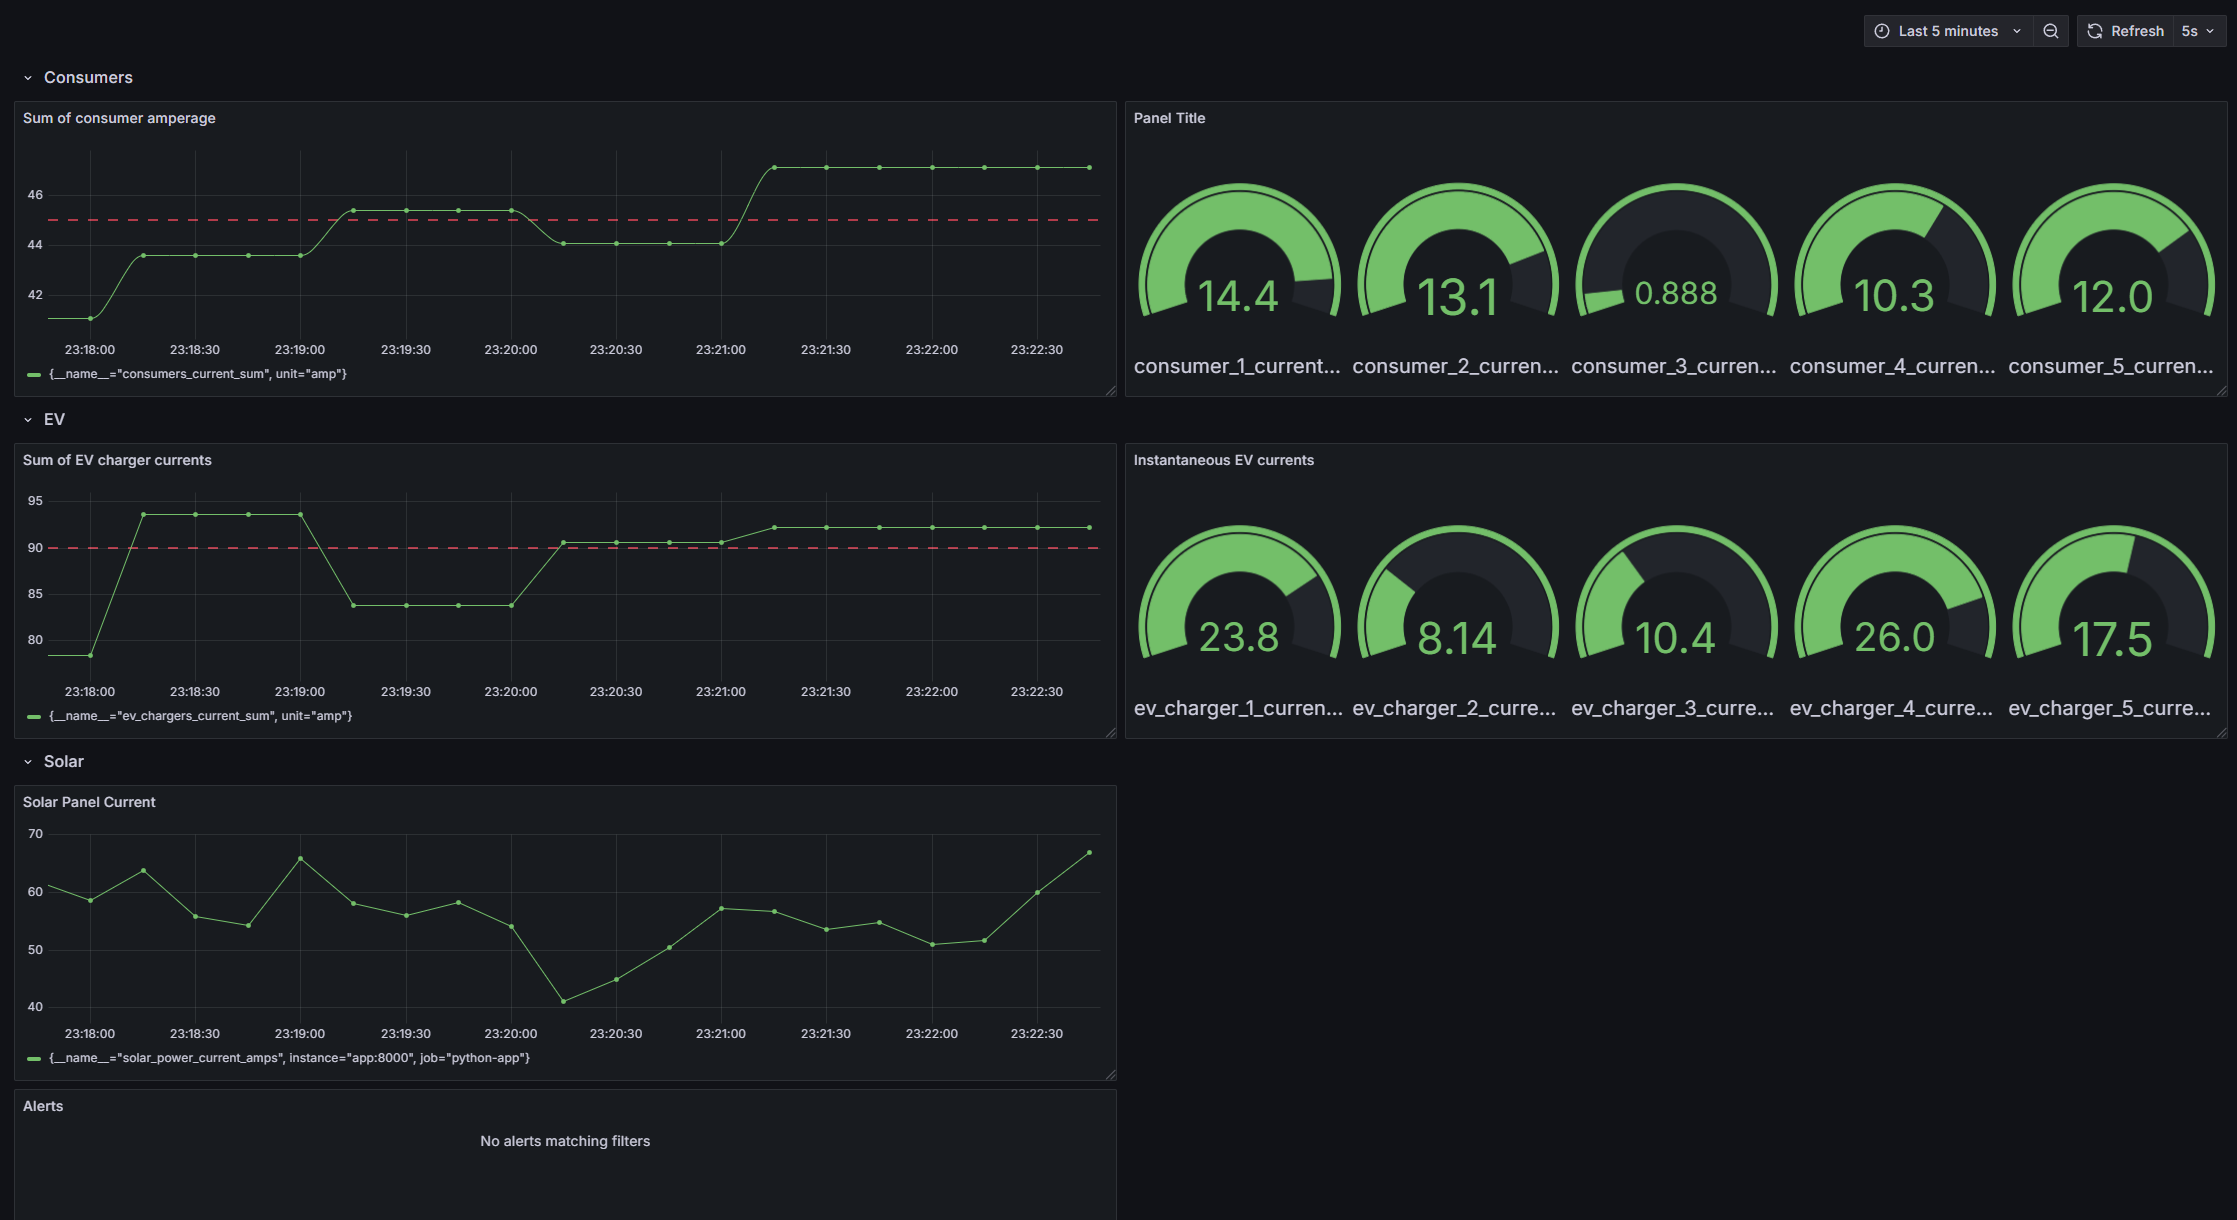
\includegraphics[width=1\textwidth, keepaspectratio]{figures/Grafana.png}
    \caption{Általam készített Grafana dashboard} 
\end{figure}
\chapter{Alkalmazás migrálása a Docker Compose-ból a Kubernetesbe}

\section{Bevezetés}

A konténerizáció nagy előnyt nyújt, mivel szabványosított, elszigetelt környezetet kínál a szoftverek futtatásához. 
A Docker Compose elterjedt a helyi, több konténert tartalmazó alkalmazásokhoz, egyszerűsítve az összekapcsolt 
szolgáltatások definiálását és futtatását. Mivel azonban sokszor skálázódásra van szükség, és olyan funkciókra, 
mint a nagy rendelkezésre állás, az automatikus skálázás és a kifinomult orkesztráció, a Kubernetes vált a konténer 
orkesztráció szabványává.

Ebben a fejezetben megmutatom, hogy az eredetileg a Docker Compose segítségével definiált rendszeremet, 
hogyan migráltam Kubernetes környezetbe. A rendszeremben a már meglévő szolgáltatások jelenek meg, mint a 
Prometheus a felügyelethez, a Grafana a vizualizációhoz, több szimulátorszolgáltatás és egy vezérlőszerver. 
Itt bemutatom a Docker Compose konfigurációk Kubernetes manifesztekbe való átforgatásának kihívásait.

\section{A Docker Compose és Kubernetes áttekintése}

Docker Compose
Ezzel több konténert tartalmazó Docker alkalmazásokat lehet definiálni és futtatni. 
Konfigurációja egy YML fájlban tárolt, ahol a szolgáltatásokat, hálózatokati kapcsolatokat, köteteket és 
függőségeket lehet megadni. A Docker Compose leegyszerűsíti a konténerek egyetlen hoszton történő orkesztrációját, 
így segíti a fejlesztést és tesztelést.

Kubernetes
A Kubernetes viszont egy robusztus, open source platform a konténerek telepítésének, 
skálázásának és üzemeltetésének automatizálására hostokon. A Kubernetes új absztrakciókat vezet be:

\begin{itemize}
    \item \textbf{Pod:} Ez a legkisebb telepíthető egység, amely egy vagy több konténert foglalnak magukba.
    
    \item \textbf{Deployment:} Állapot nélküli alkalmazások kezelésére szolgáló objektumok, amelyek olyan funkciókat kínálnak, mint a gördülő frissítések és a visszaállítás.
    
    \item \textbf{Service:} Végpontokat biztosítanak a podok eléréséhez, segítve a felfedezést és a terheléselosztást.
    
    \item \textbf{ConfigMap és Secret:} Mechanizmus a konfiguráció és az imagek szétválasztására.
    
    \item \textbf{PersistentVolumeClaim (PVC):} Absztrakció adattárolásra.
\end{itemize}

A migráció során ezeket képeztem le docker-ből k8-ba.

\begin{figure}[!ht]
    \centering
    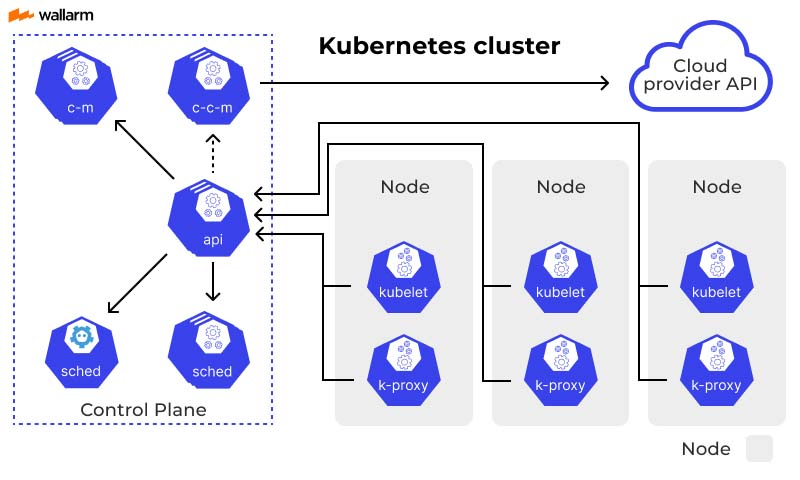
\includegraphics[width=0.8\textwidth, keepaspectratio]{figures/components-of-kubernetes.jpeg}
    \caption{Kubernetes architektúra \cite{wallarm_kubernetes_cluster}} 
\end{figure}

\section{Rendszerarchitektúrája}

A rendszer a már megismert következő részeket tartalmazza:

\begin{itemize}
    \item \textbf{Prometheus:} Egyéni prometheus.yml fájllal konfigurált idősoros adatbázis. 
    Ennek szerencsétlensége, hogy az újra konfiguráció csak újra indítással lehetséges.
    
    \item \textbf{Grafana:} Vizualizációs eszköz, ami közvetlen a Prometheushoz kapcsolódik megjelenítéséhez.
    
    \item \textbf{ESP8266 szimulátorok:} Itt épen három példány szimulálja a különböző szimulátorazonosítókkal 
    rendelkező eszközöket.
    
    \item \textbf{Breaker Simulators:} Más jellegű, de hasonló célú szimulátor.
    
    \item \textbf{Vezérlőszerver:} Lebonyolítja az eszközök közötti interakciókat, vezérlést és adatok továbbítását.
    
    \item \textbf{System Simulator:} A rendszer általános viselkedését emuláló központi szolgáltatás.
\end{itemize}

A Docker Compose alkalmazásban ezek az összetevők hálózaton és socketeken keresztül kapcsolódtak össze, 
és meghatározott végpontokon jelenítettek meg. \cite{docker_kubernetes}

\section{A Docker Compose beállítások konvertálása Kubernetes manifesztekké}

A Docker Compose-ról a Kubernetesre való áttérés magában foglalja az alkalmazás architektúrájának 
újragondolását a podok, deployement-ek, szolgáltatások és más Kubernetes objektumok szerint. \cite{kubernetes}

\subsection{Névtér- és konfigurációkezelés}

Itt létrehoztam egy névteret (pl. monitoring) ez izolációt biztosít az alkalmazás számára. 
A ConfigMap a Prometheus konfiguráció tárolására szolgál (a prometheus.yml tartalma), 
lehetővé téve a konfiguráció frissítését a konténerek image-einek újbóli legenerálása nélkül.

\begin{lstlisting}
    apiVersion: v1
kind: Namespace
metadata:
  name: monitoring
---
apiVersion: v1
kind: ConfigMap
metadata:
  name: prometheus-config
  namespace: monitoring
data:
  prometheus.yml: |-
    global:
      scrape_interval: 15s
    scrape_configs:
      - job_name: 'prometheus'
        static_configs:
          - targets: ['localhost:9090']
\end{lstlisting}

\subsection{Deployment-ek és Service-ek}

Minden szolgáltatás Docker Compose-ban egy Deployment és egy Service formájában jelenik meg a Kubernetesben. 
A Deployment kezeli az alkalmazásban a podokat, a Service ezeket a podokat teszi elérhetővé.

Például a Prometheus szolgáltatás egyetlen replikával rendelkezik. Konfigurációja a ConfigMap-ról van mountolva, 
a perzisztens adatai pedig egy PersistentVolumeClaim (PVC) segítségével tárolom. Hasonlóképpen, más szolgáltatások, 
például az ESP8266 szimulátorok és a vezérlő szerver deployement-ekké alakulnak át, amelyek környezeti változókat 
és portkonfigurációkat adnak meg.

\subsection{Perzisztens tárolók kezelése}

A Docker Compose-ban gyakran definiálnak volume-okat az adattárolására. A Kubernetesben ezt a 
PersistentVolumeClaims biztosítja. A készített rendszeremben a Prometheus, mind a Grafana perzisztens 
tárolót igényelt az adatok megőrzéséhez, amiket a PVC-k létrehozásával és konténerekhez kötésével értem el.

\begin{lstlisting}
  apiVersion: v1
kind: PersistentVolumeClaim
metadata:
  name: grafana-data
  namespace: monitoring
spec:
  accessModes:
    - ReadWriteOnce
  resources:
    requests:
      storage: 1Gi
\end{lstlisting}

\subsection{Szolgáltatások elérhetővé tétele és hálózati konfiguráció}

A Docker Compose-ban a portok hozzárendelését a konfigurációban végezzük. 
A Kubernetesben a portok meghatározást a Service-ek kezelik, ezek lehetnek 
NodePort típusúak a külső hozzáféréshez vagy ClusterIP típusúak a belső kommunikációhoz. 
A migráció során a konténerek portjait le kellett képezni a hosztokra, hogy a külső interfész 
ugyanaz maradjon az eredeti Docker Compose-hoz képest.

Például a Docker Compose-ban az 5000-es porton található vezérlő szervert egy olyan Kubernetes Service replikálja, 
amely egy adott NodePort-ot rendel hozzá, például 30050-et.

\subsection{Telepítés és tesztelés}

A Kubernetes manifeszt a kubectl apply -f paranccsal kerül alkalmazásra. Ez telepíti az összes komponenst a névtérben. 
A telepítés után a szabványos Kubernetes-parancsok (pl. kubectl get pods, kubectl logs, kubectl describe) 
a podok állapotának ellenőrzésére szolgálnak. Így iteratívan lehet tesztelni az új rendszert és később 
szolgáltatás kimaradás nélkül frissíteni.

Telepítéséhez a következő parancsot használjuk:

\begin{lstlisting}
  kubectl apply -f monitoring.yaml
\end{lstlisting}

És hogy megvizsgáljuk a telepített podokat:

\begin{lstlisting}
  kubectl get pods -n monitoring
\end{lstlisting}

\section{Nagy elérhetőségű rendszer implementációja}

Az aktív elsődleges és passzív készenléti minta csökkenti a komplexitást és 
emellett megbízható felügyeletet biztosít:

\begin{itemize}
  \item A Prometheus folyamatos adatreprodukciója mindent megőriz a második helyszínen.
  
  \item A replikán keresztül biztosított a Grafana-B azonnali használhatósága.
  
  \item Az átállást csak a DNS/szolgáltatás frissítési sebessége korlátozza.
  
  \item Ez a topológia megfelel a megbízhatósági céloknak a monitorozási környezetbe.
  
\end{itemize}

\begin{figure}[!ht]
  \centering
  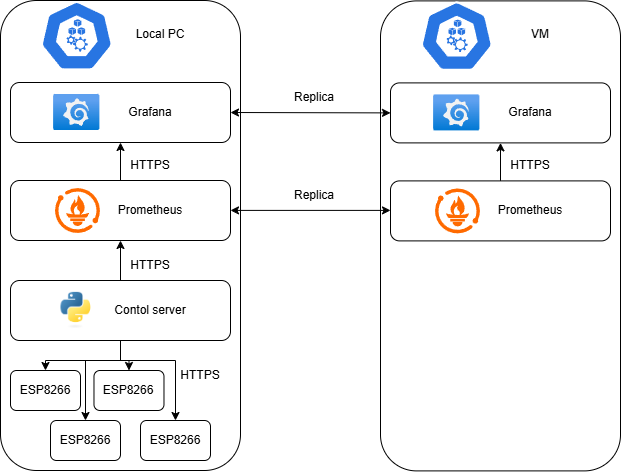
\includegraphics[width=0.8\textwidth, keepaspectratio]{figures/kubernetes.png}
  \caption{Hibrid kubernetes topológia}
\end{figure}

A Prometheus-A minden célpontot lekérdez, és elvégzi az összes értékelést.
A Prometheus-B távoli írást kap A-tól (A hálózat felesleges terhelésének 
elkerülése érdekében nem scrapel közvetlen).
A Grafana-B csatlakozik a Prometheus-B-hez, és a dashboardokat inen frissíti 
(ez közvetlenül nem érhető el).
Egyetlen DNS név mutat az A ingressre. A Kubernetes és egy külső állapotellenőrzés 
frissíti a DNS-t a B oldalra, amikor az A leáll.

\subsection{Replikák megvalósítása}

A VM-n a prometheus konfigurációja a következő képen történik.

\begin{lstlisting}
  apiVersion: apps/v1
kind: Deployment
metadata:
  name: prometheus-b
  namespace: monitoring
spec:
  replicas: 1
  selector: { matchLabels: { app: prometheus-b } }
  template:
    metadata: { labels: { app: prometheus-b } }
    spec:
      nodeSelector: { site: "b" }
      containers:
      - name: prometheus
        image: prom/prometheus:v2.49
        args:
          - --config.file=/etc/prometheus/prometheus.yml
          - --web.enable-lifecycle
        volumeMounts:
          - name: data
            mountPath: /prometheus
        readinessProbe: { httpGet: { path: /-/ready, port: 9090 } }
      volumes:
      - name: data
        persistentVolumeClaim:
          claimName: prometheus-b-data
---
kind: PersistentVolumeClaim
metadata:
  name: prometheus-b-data
  namespace: monitoring
spec:
  accessModes: [ReadWriteOnce]
  storageClassName: cloud-ssd
  resources: { requests: { storage: 50Gi } }
\end{lstlisting}

Az eredeti A prometheus-ból pedig a B-be folyamatosan írunk.

\begin{lstlisting}
  remote_write:
- url: http://prometheus-b.monitoring.svc.cluster.local:9090/api/v1/write
  queue_config:
    capacity: 10000
    max_shards: 5
    max_samples_per_send: 1000
    batch_send_deadline: 5s
\end{lstlisting}

A grafana megvalósítása során igazából csak egy ugyanolyan deployement-et hozunk létre.
Ez egy másolat a másikról amire ha kell áttudunk bármikor térni.

\begin{lstlisting}
  spec:
  replicas: 1
  template:
    metadata: { labels: { app: grafana-b } }
    spec:
      nodeSelector: { site: "b" }
      containers:
      - name: grafana
        image: grafana/grafana:11.0.0
        env:
          - name: GF_DATABASE_URL     # same secret as primary
            valueFrom: { secretKeyRef: { name: grafana-db, key: db_url } }
          - name: GF_SECURITY_SECRET_KEY
            valueFrom: { secretKeyRef: { name: grafana-db, key: secret } }
        readinessProbe:
          httpGet: { path: /api/health, port: 3000 }
\end{lstlisting}

\subsection{KubeADM}

A projektemben a kubeadm-re támaszkodtam, hogy kubernetes klasztert készítsek a linux vm-et bevonva. 
Ez megkönnyítette a folyamatot mert magasabb színtű tervezésre volt csak szükség és ez megoldotta magától 
az alacsonyabb szintű problémákat.

\begin{lstlisting}
  sudo kubeadm init --config=/etc/kubeadm/config.yaml
\end{lstlisting}

Az inicializálás után csak egy tokent kellett adni a nodenak, hogy csatlakozzon a clusterhez.
Ezután a a további folyamatokat kezelte is a Kubeadm.

\begin{lstlisting}
  sudo kubeadm join 10.200.0.1:6443 \
    --token <token> \
    --discovery-token-ca-cert-hash sha256:<hash>
\end{lstlisting}

Ennek köszönhetően egy hasonló rendszerben, ha a egy node meghibásodik akkor a másik átveszi a helyét és felhasználói oldalról
nem érzünk kiesést. A helyre állítás során, pedig csak egy parancsot kell kiadnunk:

\begin{lstlisting}
  kubeadm join
\end{lstlisting}

Ezután újra csatlakoztattuk is a node-ot és újonnan felépíthetjük a clusterben.
\chapter{Felhasználói felület}

\section{Szöveges be- és kimenetek a szimulációhoz}

\subsection{Cél és áttekintés}
A rendszer szöveges alapú beállításra és eredménygyűjtésre alkalmas. 
A cél, hogy a szimuláció \emph{kiegészítő eszközök} (pl.\ curl, CSV-konverzió) nélkül, 
egyszerű szövegfájlokkal legyen vezérelhető és kiértékelhető.

\noindent Rövid összefoglaló:
\begin{itemize}
  \item \textbf{Bemenetek:} \texttt{thresholds.txt}, \texttt{esp\{1..3\}\_schedule.txt}, \texttt{sim\_control.txt}
  \item \textbf{Kimenet/napló:} \texttt{output.txt} (idősoros; egy sor = egy vezérlési ciklus)
  \item \textbf{Webes felület:} ``Dev Panel'' (localhost:8080) a fájlok szerkesztéséhez, generálásához, 
  letöltéséhez, a futás indításához/megállításához, az idő nullázásához és a napló törléséhez.
\end{itemize}

\subsection{Bemeneti szövegfájlok}

\subsubsection{\texttt{thresholds.txt} -- küszöbök és maximum megengedhető áram}
A vezérlő szerver minden ciklusban beolvassa. Kulcs--érték párok, tizedes ponttal:
\begin{verbatim}
# Küszöbértékek a vezérlő szerverhez
BREAKER_MAX_TOTAL=65.0    # [A] - Megszakító lekapcsolási áram
BREAKER_MIN_TOTAL=35.0    # [A] - Megszakító bekapcsolási áram
ALLOC_MAX_TOTAL=95.0      # [A] - Max áram érték
\end{verbatim}

\noindent Megjegyzések:
\begin{itemize}
  \item A \emph{megszakítók} (breakerek) logikája az \emph{aktuálisan mért hatásos} összáramhoz 
  viszonyít (\texttt{BREAKER\_MAX\_TOTAL}, \texttt{BREAKER\_MIN\_TOTAL}).
  \item A SIM-ekre küldött korlátok (cap) a \emph{nyers igényekből} számítódnak \emph{max-min fair} elv 
  szerint, az \texttt{ALLOC\_MAX\_TOTAL} keret figyelembevételével.
\end{itemize}

\subsubsection{\texttt{esp\{x\}\_schedule.txt} -- idősoros bemenet}
Formátum: időpillanat másodpercben + kívánt áram (A). A menetrend \emph{lépcsős}: a legutóbbi időponthoz 
tartozó érték érvényes a következő megadásig.
\begin{verbatim}
# seconds  amps
0         1.0
30        2.5
120       0.8
\end{verbatim}
\noindent Irányelvek: tizedes elválasztó pont; tetszőleges szóköz; a sorok idő 
szerint rendezve mint minden szöveges ki- és bemeneti file-ban.

\subsubsection{\texttt{sim\_control.txt} -- futtatási állapot}
Egyetlen szó: \texttt{RUNNING} vagy \texttt{STOPPED} (Az alapértelmezés \texttt{STOPPED}). 
A SIM-ek ``virtuális órája'' csak \texttt{RUNNING} állapotban megy.

\subsection{Kimeneti szövegfájl}

\subsubsection{\texttt{output.txt} -- idősoros kimenet}
A vezérlő minden ciklusban \emph{egy sort} ír. A fájl alapértelmezetten \emph{append-only} 
a véletlen szerkesztést elkerülendő; a Dev Panel ``Clear output.txt'' művelete törli amennyiben ez szükséges, 
és a vezérlő legközelebb automatikusan újra létrehozza a fejlécet.

\noindent Formátum: \texttt{kulcs=érték} párok szóközzel elválasztva.
\begin{verbatim}
# One record per line; fields are key=value separated by spaces
timestamp=1758199200 sim_state=RUNNING sum_current_amps=5.7 \
alloc_max_total_amps=6.0 max_total_amps=6.0 min_total_amps=1.0 \
sims=esp1:raw=2.0,effective=2.0,cap=2.0|esp2:raw=1.7,effective=1.7,
cap=2.0|esp3:raw=2.5,effective=2.0,cap=2.0 \
breakers=brk1:on,brk2:on
\end{verbatim}

\noindent Kulcsok a kimeneti file-ban:
\begin{itemize}
  \item \texttt{timestamp} -- UNIX időpecsét (s).
  \item \texttt{sim\_state} -- globális állapot: \texttt{RUNNING}/\texttt{STOPPED}.
  \item \texttt{sum\_current\_amps} -- mért hatásos összáram (cap után).
  \item \texttt{alloc\_max\_total\_amps} -- allokációs keret (A).
  \item \texttt{max\_total\_amps} / \texttt{min\_total\_amps} -- breaker küszöbök (legacy nevek).
  \item \texttt{sims} -- \texttt{|} jellel szeparált lista SIM-enként:\\
  \texttt{espX:raw=\dots, effective=\dots, cap=\dots}\\
  ahol \texttt{raw} = menetrendi igény, \texttt{effective} = tényleges áram, \texttt{cap} = küldött maximum.
  \item \texttt{breakers} -- megszakítók állapota \texttt{on}/\texttt{off}, vesszővel elválasztva.
\end{itemize}

\subsection{Időkezelés és futtatás}
\begin{itemize}
  \item \textbf{Virtuális idő:} minden SIM saját menetrendi ideje csak \texttt{RUNNING} állapotban növekszik.
  \item \textbf{STOPPED} módban a SIM-ek ideje megáll; a vezérlő nem küld új cap-et és 
  nem kapcsolgat megszakítót, csak mér és naplóz.
  \item \textbf{Reset (t=0):} a Dev Panel ``Reset sim time (t=0)'' gombja az összes 
  SIM virtuális idejét nullázza (a panel előbb STOP-ra állít, majd resetel).
\end{itemize}

\subsection{Reprodukálhatóság és feldolgozhatóság}
A bemenetek (küszöbök, menetrendek, futtatási állapot) verziózhatók és mellékelhetők. 
A kimeneti \texttt{output.txt} önleíró; minden rekord tartalmazza az adott ciklus lényeges paramétereit. 
A formátum egyszerűen feldolgozható bármely nyelven (kulcs=érték párok; \texttt{sims} és \texttt{breakers} 
mezők jól definiált szeparátorokkal).

\subsection{Rövid példa -- beállítás $\rightarrow$ kimenet (részlet)}

\paragraph{thresholds.txt}
\begin{verbatim}
BREAKER_MAX_TOTAL=9.0
BREAKER_MIN_TOTAL=2.0
ALLOC_MAX_TOTAL=9.0
\end{verbatim}

\paragraph{esp1\_schedule.txt}
\begin{verbatim}
# seconds  amps
0  50
60 10
\end{verbatim}

\paragraph{esp2\_schedule.txt}
\begin{verbatim}
0  50
60 10
\end{verbatim}

\paragraph{esp3\_schedule.txt}
\begin{verbatim}
0  50
60 100
\end{verbatim}

\noindent Várható kiosztás a 0--60 s szakaszban: mindhárom SIM korlátozott, 
mivel az igény 150 A $>$ 9 A. 60 s után az 
igények \texttt{[10, 10, 100]} $\Rightarrow$ kiosztás \texttt{[10, 10, 70]}. A \texttt{cap} és 
az \texttt{effective} értékek ennek megfelelően jelennek meg az \texttt{output.txt}-ben.

% =====================================================================
\chapter{Max--min fair (water-filling) elosztás}

\section{Elméleti háttér és cél}

\subsection{Motiváció és cél}
A szimulált fogyasztók  áramigénye (\(d_i\)) időben változik. 
Adott egy globális, maximum áramérték \(\,B=\texttt{ALLOC\_MAX\_TOTAL}\,\) amperben, 
ennél a tényleges összáram nem lehet nagyobb. A cél egy olyan kiosztás \(\,a_i\) meghatározása, amely
(i) nem lépi túl az egyes igényeket (\(0\le a_i\le d_i\)),
(ii) a teljes kereten belül marad (\(\sum_i a_i \le B\)),
(iii) és \emph{fair} a kis igényűekkel szemben, azaz a kis igények teljesülnek először, a 
fennmaradó kapacitás pedig egyenlő alapról oszlik meg.

\subsection{Definíció (max--min fair)}
Egy \(\,a=(a_1,\dots,a_n)\) kiosztás \emph{max--min fair}, ha bármely más megengedett \(\,y\) esetén, 
ha létezik \(i\) úgy, hogy \(y_i > a_i\), akkor létezik \(j\) olyan, hogy \(a_j \le a_i\) és \(y_j < a_j\). 
Intuíció: csak a \emph{már kisebb} részesedésűek rovására lehet növelni bárki juttatását. \cite{wiki:max-min-fairness}

\subsection{Feltöltés (water-filling)}
A max--min fair kiosztás felírható egyetlen paraméterrel:
\begin{equation}
  a_i = \min\{\,d_i,\ \lambda\,\}, \qquad \text{ahol }\ \sum_{i=1}^n \min\{d_i,\lambda\} \;=\; B.
\end{equation}
A \(\lambda\) \emph{vízszint} úgy választandó, hogy a keret pont kiteljen (vagy ha \( \sum_i d_i < B\), 
akkor \(\lambda\ge \max_i d_i\), vagyis nincs korlát).

\subsection{Algoritmus és bonyolultság}
Gyakorlati, determinisztikus eljárás (progresszív töltés):
\begin{enumerate}
  \item Rendezzük az igényeket növekvő sorrendbe: \(d_{(1)} \le \dots \le d_{(n)}\).
  \item Iteráljuk \(k=1..n\): feltételezzük, hogy az első \(k\) igény teljesül (\(a_{(i)}=d_{(i)}\), \(i\le k\)), 
  és a maradék \(B_k = B - \sum_{i=1}^k d_{(i)}\) egyenlő szinten oszlik meg a még nyitott \(n-k\) elemre. 
  A jelölt vízszint: \(\lambda_k = B_k/(n-k)\).
  \item Ha \(\lambda_k \le d_{(k+1)}\), megtaláltuk a vízszintet: az összes hátralévő \(a_{(i)}=\lambda_k\) 
  (és a korábbiak \(d_{(i)}\)).
  \item Ha minden \(d_{(i)}\) teljesül és még marad keret, akkor nincs korlátozás: \(a_i=d_i\).
\end{enumerate}
A rendezés miatt az időbonyolultság \(O(n\log n)\). A megvalósított vezérlőben egy ekvivalens, 
iteratív \emph{progresszív} algoritmus fut, amely kis elemszámon szintén gyors és stabil.

\begin{figure}
    \centering
    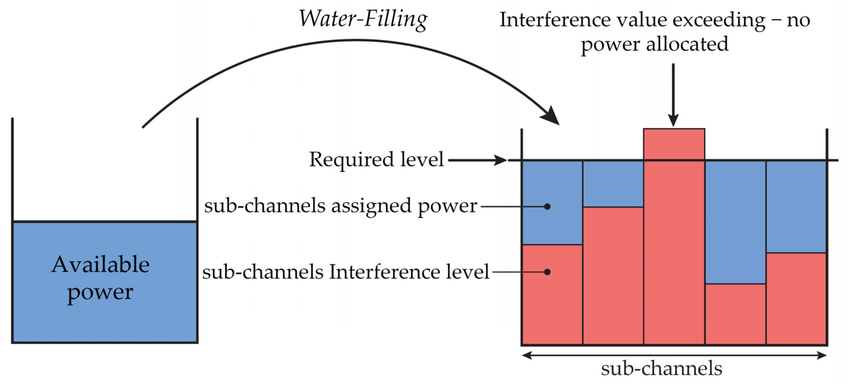
\includegraphics[width=1\textwidth]{figures/Principle-of-Water-Filling-algorithm-76.png}
    \caption{Water-filling elve telekomunikációban. \cite{Slacik2021Sensors}}
    \label{fig:water-filling}
\end{figure}

\subsection{Tulajdonságok}
\begin{itemize}
  \item \textbf{Egyenlő szint elve:} a \(\lambda\) alatti igények teljes, a \(\lambda\) 
  felettiek \(\lambda\)-ig kapnak. Így a kis igényűek sosem szenvednek hátrányt.
  \item \textbf{Monotonitás:} ha a keret \(B\) nő, akkor \(\lambda\) nem csökken, és senki kiosztása nem csökken.
  \item \textbf{Határhelyzetek:} ha \(\sum_i d_i \le B\) → nincs cap (végtelen korlát). Ha \(B=0\) → minden \(a_i=0\).
\end{itemize}

\section{A vezérlőben alkalmazott megvalósítás}

\subsection{Kapcsolat a rendszer komponenseivel}
A vezérlő igényekből (\texttt{raw\_current}) számolja a limiteket a fenti elv szerint 
a \texttt{ALLOC\_MAX\_TOTAL} kereten. A \emph{megszakító} (breaker) logika ettől független, 
a \emph{mért, tényleges} áramhoz viszonyít (\texttt{BREAKER\_MAX\_TOTAL}, \texttt{BREAKER\_MIN\_TOTAL}) 
biztonsági rétegként.

\subsection{Példák}
\paragraph{Klasszikus példa.}
\(d=[10,10,100]\), \(B=90\) \(\Rightarrow\) \(a=[10,10,70]\) (a két kicsi teljesül, a maradék egy szinten oszlik meg).
\paragraph{Vegyes igények.}
\(d=[3,8,8,20]\), \(B=25\) \(\Rightarrow\) rendezve az első igény (3) teljesül, a maradék \(22\) 
három felé oszlik: \(a=[3,\,7.33,\,7.33,\,7.33]\) A.

\subsection{Implementációs részletek}
A limitek csak \(\pm 10^{-3}\) A változás felett frissülnek a fogyasztók felé (zajcsillapítás), 
a „nincs korlát” állapotot nagy \(\texttt{INF\_CAP}\) érték reprezentálja. Ha a nyers igény összeg a keret alá esik, 
a limitek feloldódnak.

% =====================================================================

\chapter{Fejlesztői panel (Dev Panel)}

\section{Cél és szerep}
A Dev Panel egy könnyű használatú webes felület, amely a szöveges bemenetek és kimenetek kezelését, 
a futtatás indítását/megállítását, az idő nullázását és a napló törlését teszi lehetővé. Célja 
a \emph{gyors kísérletezés} és a \emph{reprodukálható} tesztfutások támogatása külön eszközök nélkül.

\section{Architektúra áttekintése}
A panel egy Flask-alapú backendből (\texttt{/api/*}) és statikus frontendből (HTML+CSS+JS) áll. 
A backend közvetlenül a \texttt{./data} mappában található fájlokat kezeli, 
és hálózaton hívja az esp-t szimuláló konténerek végpontjait. A vezérlő külön, 
a saját portján (\(8000\)) fut; a Prometheus és Grafana eléréséhez gyorslinkek állnak rendelkezésre.

\section{Fő funkciók és munkamenet}
\paragraph{Start/Stop.} A \texttt{sim\_control.txt} fájlba írja a panel 
a \texttt{RUNNING} vagy \texttt{STOPPED} értéket. STOP módban az esp szimulátorok virtuális ideje megáll, 
a vezérlő nem küld max értékeket és nem kapcsol megszakítókat, csak mérést és naplózást végez.
\paragraph{Reset (t=0).} A panel a STOP beállítás után meghívja minden esp szimulátor \texttt{/reset\_time} 
végpontját, a virtuális idejük nulláról indul újra.
\paragraph{Clear output.txt.} A \texttt{data/output.txt} törlése. A vezérlő a következő ciklusban 
automatikusan újra létrehozza a fejlécet és folytatja a naplózást.
\paragraph{Thresholds szerkesztés.} A \texttt{thresholds.txt} beolvasása/írása a panelről: 
\texttt{BREAKER\_MAX\_TOTAL}, \texttt{BREAKER\_MIN\_TOTAL}, \texttt{ALLOC\_MAX\_TOTAL}.
\paragraph{Menetrend-generátor.} Konstans, fel- és lefutás, lépcső, szinusz és random walk idősorok képezhetők 
a \texttt{esp\{x\}\_schedule.txt} fájlokba (formátum: \texttt{seconds\ \ \ amps}). 
A generált tartalom előnézetben ellenőrizhető.
\paragraph{Raw editor \& Letöltés.} Tetszőleges bemeneti fájl közvetlen szerkeszthető; 
az \texttt{output.txt} csak olvasható. Minden be- és a kimenet letölthető megőrzéshez.

\section{Backend API (elérések)}
\begin{center}
\begin{tabular}{ll}
\hline
\textbf{Végpont} & \textbf{Funkció} \\
\hline
\texttt{GET\ /api/read?name=...} & Fájl beolvasása \\
\texttt{POST\ /api/write} & Fájl írása \\
\texttt{GET\ /api/download?name=...} & Közvetlen letöltés \\
\texttt{GET\ /api/sim\_state} & Globális állapot lekérdezése \\
\texttt{POST\ /api/sim\_state} & RUNNING/STOPPED beállítása \\
\texttt{POST\ /api/clear\_output} & \texttt{output.txt} törlése \\
\texttt{POST\ /api/reset\_sim\_time} & Minden szimulátor időnullázása \\
\hline
\end{tabular}
\end{center}

\section{Biztonsági és korlátok}
A panel \emph{belső} használatra készült. Nincs többfelhasználós jogosultság- és CSRF-kezelés; 
éles környezetben ezeket pótolni szükséges. A fájlműveletek engedélyezett listához kötöttek, 
a végpontok nem tesznek lehetővé tetszőleges fájlhozzáférést.

\section{Kiterjeszthetőség}
A panel könnyen bővíthető új be- és kimenetekkel: pl.\ súlyozott fair-elosztás bemenete (\texttt{weights.txt}), 
előre definiált menetrend-sablonok, vagy beépített grafikon a \texttt{output.txt} vizualizálására. 
A funkcionalitás változtatása különösen egyszerű, mivel az állapot \emph{szöveges fájlokban} 
van deklarálva.

\begin{figure}
    \centering
    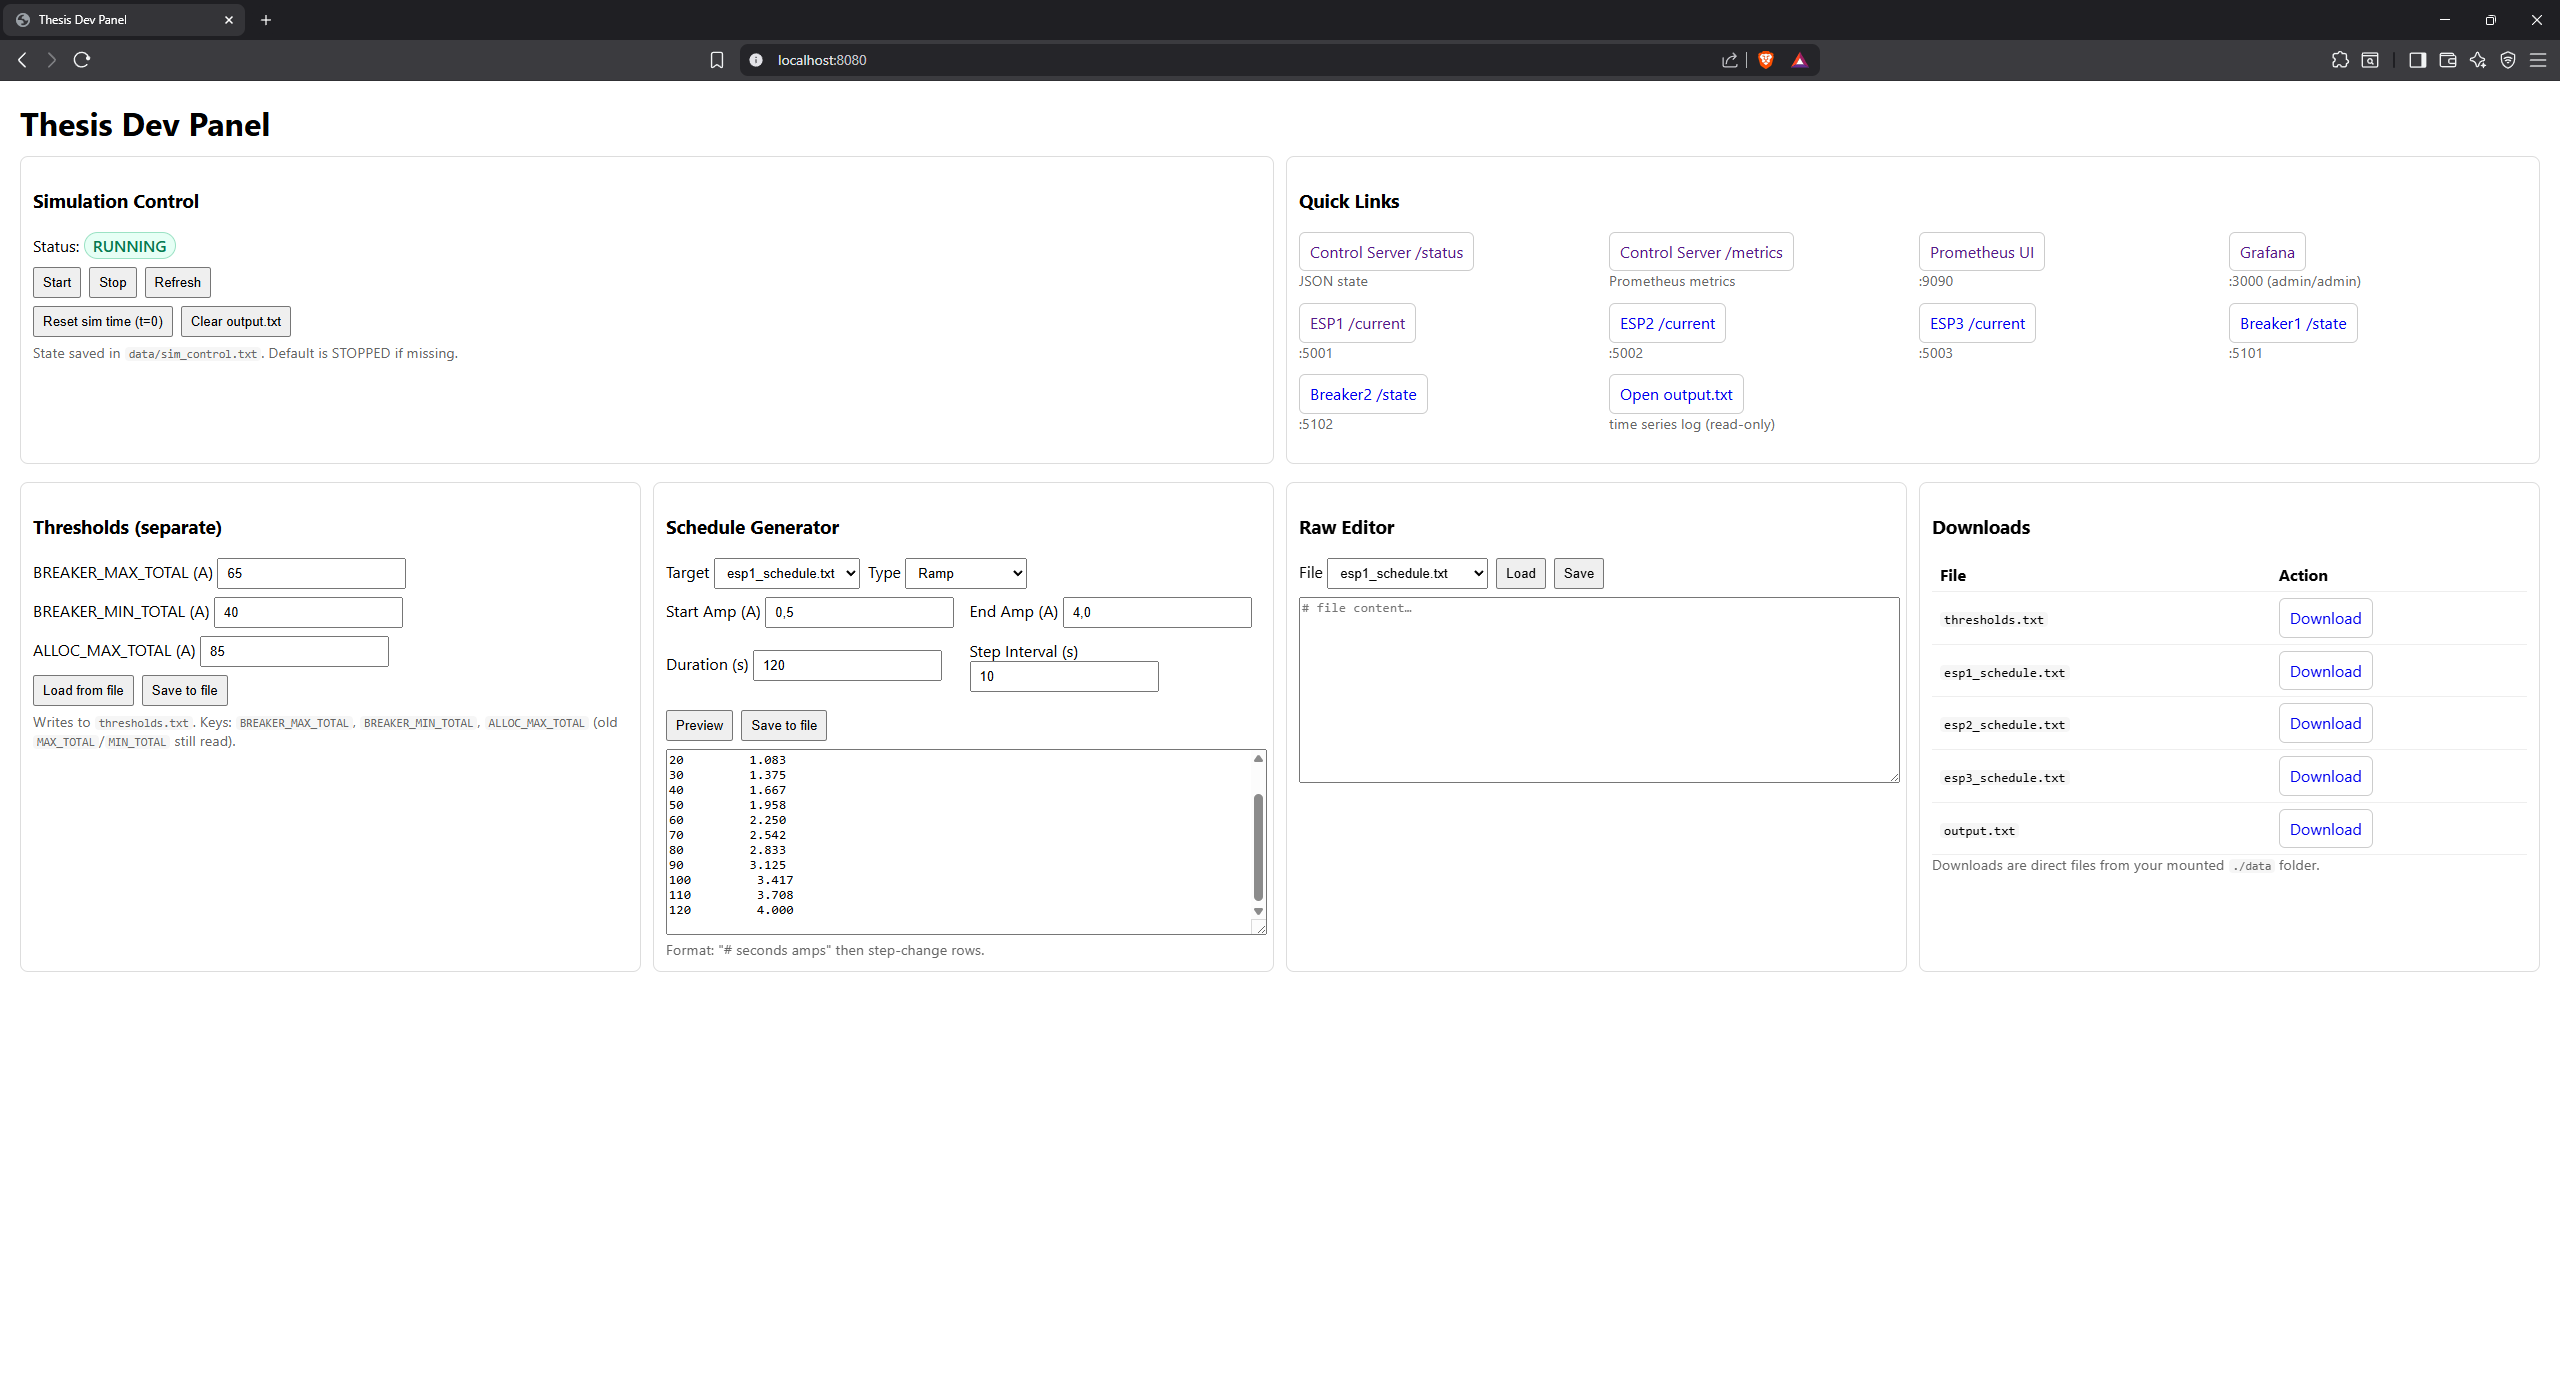
\includegraphics[width=1\textwidth]{figures/devpanel.png}
    \caption{Devpanel}
    \label{fig:devpanel}
\end{figure}


% Acknowledgements
%~~~~~~~~~~~~~~~~~~~~~~~~~~~~~~~~~~~~~~~~~~~~~~~~~~~~~~~~~~~~~~~~~~~~~~~~~~~~~~~~~~~~~~
%%----------------------------------------------------------------------------
\chapter*{\koszonetnyilvanitas}\addcontentsline{toc}{chapter}{\koszonetnyilvanitas}
%----------------------------------------------------------------------------

Ez nem kötelező, akár törölhető is. Ha a szerző szükségét érzi, itt lehet köszönetet nyilvánítani azoknak, akik hozzájárultak munkájukkal ahhoz, hogy a hallgató a szakdolgozatban vagy diplomamunkában leírt feladatokat sikeresen elvégezze. A konzulensnek való köszönetnyilvánítás sem kötelező, a konzulensnek hivatalosan is dolga, hogy a hallgatót konzultálja. TODO ha kéne köszönet


% List of Figures, Tables
%~~~~~~~~~~~~~~~~~~~~~~~~~~~~~~~~~~~~~~~~~~~~~~~~~~~~~~~~~~~~~~~~~~~~~~~~~~~~~~~~~~~~~~
%\listoffigures\addcontentsline{toc}{chapter}{\listfigurename}
%\listoftables\addcontentsline{toc}{chapter}{\listtablename}


% Bibliography
%~~~~~~~~~~~~~~~~~~~~~~~~~~~~~~~~~~~~~~~~~~~~~~~~~~~~~~~~~~~~~~~~~~~~~~~~~~~~~~~~~~~~~~
\addcontentsline{toc}{chapter}{\bibname}
\bibliography{bib/mybib}


% Appendix
%~~~~~~~~~~~~~~~~~~~~~~~~~~~~~~~~~~~~~~~~~~~~~~~~~~~~~~~~~~~~~~~~~~~~~~~~~~~~~~~~~~~~~~
%%----------------------------------------------------------------------------
\appendix
%----------------------------------------------------------------------------
\chapter*{\fuggelek}\addcontentsline{toc}{chapter}{\fuggelek}
\setcounter{chapter}{\appendixnumber}
%\setcounter{equation}{0} % a fofejezet-szamlalo az angol ABC 6. betuje (F) lesz
\numberwithin{equation}{section}
\numberwithin{figure}{section}
\numberwithin{lstlisting}{section}
%\numberwithin{tabular}{section}

%----------------------------------------------------------------------------
\section{PÉLDA}
%----------------------------------------------------------------------------
\begin{figure}[!ht]
\centering
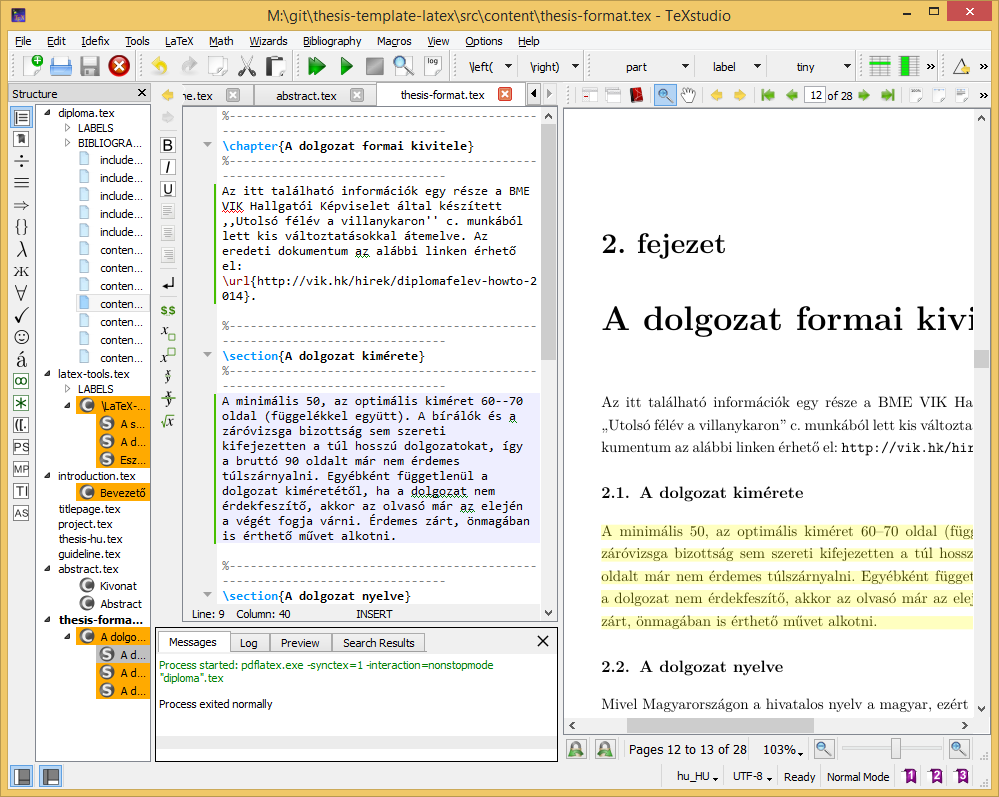
\includegraphics[width=150mm, keepaspectratio]{figures/TeXstudio.png}
\caption{A TeXstudio \LaTeX-szerkesztő.} 
\end{figure}

%----------------------------------------------------------------------------
\clearpage

%\label{page:last}
\end{document}
